%%%%%%%%%%%%%%%%%%%%%%% file template.tex %%%%%%%%%%%%%%%%%%%%%%%%%
%
% This is a general template file for the LaTeX package SVJour3
% for Springer journals.          Springer Heidelberg 2010/09/16
%
% Copy it to a new file with a new name and use it as the basis
% for your article. Delete % signs as needed.
%
% This template includes a few options for different layouts and
% content for various journals. Please consult a previous issue of
% your journal as needed.
%
%%%%%%%%%%%%%%%%%%%%%%%%%%%%%%%%%%%%%%%%%%%%%%%%%%%%%%%%%%%%%%%%%%%
%
% First comes an example EPS file -- just ignore it and
% proceed on the \documentclass line
% your LaTeX will extract the file if required
\begin{filecontents*}{example.eps}
%!PS-Adobe-3.0 EPSF-3.0
%%BoundingBox: 19 19 221 221
%%CreationDate: Mon Sep 29 1997
%%Creator: programmed by hand (JK)
%%EndComments
gsave
newpath
  20 20 moveto
  20 220 lineto
  220 220 lineto
  220 20 lineto
closepath
2 setlinewidth
gsave
  .4 setgray fill
grestore
stroke
grestore
\end{filecontents*}
% %
\RequirePackage{fix-cm}
%
\documentclass{svjour3}                     % onecolumn (standard format)
%\documentclass[smallcondensed]{svjour3}     % onecolumn (ditto)
%\documentclass[smallextended]{svjour3}       % onecolumn (second format)
%\documentclass[twocolumn]{svjour3}          % twocolumn
%
\smartqed  % flush right qed marks, e.g. at end of proof
%
\usepackage{graphicx}
%
% \usepackage{mathptmx}      % use Times fonts if available on your TeX system
%
% insert here the call for the packages your document requires
%\usepackage{latexsym}
\setlength{\textheight}{9.05343in}
\usepackage{pgfplots}
\usetikzlibrary{backgrounds,automata}
\pgfplotsset{compat=newest}
\usepackage{epsfig}
\usepackage{array}
\usepackage{float}

\let\proof\relax
\let\endproof\relax
\usepackage{amsthm,amssymb,graphicx,graphicx,multirow,amsmath,color}
\usepackage{caption}
\usepackage{tikz}
\usepackage{algpseudocode}
\usepackage{algorithm}
\captionsetup{belowskip=-4pt}
\usetikzlibrary{plotmarks,shapes.geometric,arrows}
\usetikzlibrary{patterns}
\usetikzlibrary{calc,positioning,fit,backgrounds}
\usetikzlibrary{shapes,snakes}
\usetikzlibrary{intersections,positioning}
\usepackage{subcaption}
\DeclareMathOperator{\E}{\mathbb{E}}
\usepackage{appendix}
%\usepackage[lofdepth,lotdepth]{subfig}
%\usepackage{subfig}
\usepackage[english]{babel}
\usepackage[noadjust]{cite}
\addtolength{\topmargin}{0.3in}
%\usepackage{hyperref}
%\usepackage[T1]{fontenc}
\usepackage{url}
\usepackage[margin=1in]{geometry}
%\doublespacing
%\pagenumbering{arabic}
\include{notation2}

\def\st#1{{\color{red} #1 }}
\def\rep#1{{\color{blue} #1 }}
% \renewcommand{\H}{\textbf{H}}
% \newcommand{\Q}{\textbf{Q}}
% \newcommand{\y}{\textbf{y}}
% \newcommand{\x}{\textbf{x}}
% \newcommand{\No}{\textbf{n}}
% \newcommand{\W}{\textbf{W}}
% \newcommand{\Lb}{\textbf{L}}
% \newcommand{\I}{\textbf{I}}
% \newcommand{\ie}{\textit{i.e.}}
% \newcommand{\sinr}{\text{SINR}}
% \newcommand{\ber}{\text{BER}}
% \newcommand{\snr}{\text{SNR}}
% \newcommand{\one}{1}
%\newcommand{\ceil}[1]{\lceil #1\rceil}
\def\argmin{\operatorname{arg~min}}
\def\argmax{\operatorname{arg~max}}
\def\figref#1{Fig.\,\ref{#1}}%
\def\E{\mathbb{E}}
\def\Y{\mathbf{Y}}
\def\H{\mathbf{H}}
\def\B{\mathbf{B}}
\def\Rb{\mathbf{R}}
\def\Eb{\mathbf{E}}
\def\Lb{\mathbf{L}}
\def\X{\mathbf{X}}
\def\Nb{\mathbf{N}}
\def\W{\mathbf{W}}
\def\dk{\mathbf{d}_k}
\def\u{\upsilon}
\def\EE{\mathbb{E}^{!o}}
\def\P{\mathbb{P}}
\def\pzf{\mathtt{P}_{\mathtt{PZF}}}
\def\pmmse{\mathtt{P}_{\mathtt{MMSE}}}
\def\PP{\mathcal{P}}
\def\ie{{\em i.e.}}
\def\eg{{\em e.g.}}
\def\V{\operatorname{Var}}
\def\erfc{\operatorname{erfc}}
\def\erf{\operatorname{erf}}
\def\opt{\mathrm{opt}}
\def\R{\mathbb{R}}
\def\No{\mathbf{n}}
\def\Z{\mathbb{Z}}
\def\calN{\mathcal{N}}
\def\calM{\mathcal{M}}
\def\calC{\mathcal{C}}
\def\calT{\mathcal{T}}
\def\L{\mathcal{L}}
\def\LL{\mathcal{L}^{!o}}
\def\BB{\mathbf{B}}
\def\one{\mathbf{1}}
\def\var{\operatorname{var}}
\def\out{\mathrm{out}}
\def\cid{\stackrel d\rightarrow}
\def\supp{\operatorname{supp}}
\def\rg{r_{\mathrm G}}
\def\Nin{N^{\mathrm{in}}}
\def\Nout{N^{\mathrm{out}}}
\def\i{\mathbf{1}}
\def\v{\mathbf{v}}
\def\us{\mathbf{u}}
\def\B{\mathcal{B}}


% specifically for this paper.

\def\d{\mathrm{d}}
\def\t{\theta}
\def\k{\mathtt{\kappa}}
\def\m{\mathtt{\mu}}
\def\p{\mathtt{P}}
\def\x{\mathbf{x}}
\def\dx{\mathbf{d}}
\def\s{\mathbf{s}}
\def\y{\mathbf{y}}
\def\z{\mathtt{z}}
\def\I{\mathbf{I}}
\def\ps{\mathtt{P_{sd}}}
\def\F{\mathtt{F_{sd}}}
\def\f{\mathtt{f_{h}} }

\def\pa{\mathtt{P}}
\def\C{\mathtt{C}}
\def\G{\mathcal{G}}
\def\o{\hat{o}}
\def\Q{\mathbf{Q}}

\def\a{d}
\def\sp{\rho^{(2)}_\eta}
\def\som{\mathcal{K}_\eta}

\def\tp{\rho^{(3)}}


\def\l{\ell}
\newcommand{\fad}[2]{\ensuremath{\mathtt{h}_{#1}[#2]}}
\newcommand{\h}[1]{\ensuremath{\mathtt{h}_{#1}}}
\newcommand{\hh}[1]{\ensuremath{\mathbf{h}_{#1}}}


\def\EP{\mathbb{E}^{!o}}
\def\T{\theta}
\def\sinr{\mathtt{SINR}}
\def\snr{\mathtt{SNR}}
\def\sir{\mathtt{SIR}}
\def\ber{\mathtt{BER}}

%% Definitions
%\newtheorem{lemma}{Lemma}{}
\newtheorem{thm}{Theorem}
%\newtheorem{theorem}{Theorem}
\newtheorem{prop}{Proposition}
\newtheorem{cor}[thm]{Corollary}
\newtheorem{conj}[thm]{Conjecture} 

\newtheorem{defi}[thm]{Definition}
%\newtheorem{definition}[thm]{Definition}


%\fnmsep
%\renewcommand{\baselinestretch}{1.2} %for double-spaced, use 1.6
% etc.
%
% please place your own definitions here and don't use \def but
% \newcommand{}{}
%
% Insert the name of "your journal" with
% \journalname{myjournal}
%

% \makeatletter
% \let\@fnsymbol\@arabic
% \makeatother


\begin{document}

\title{%about the article that should go on the front page should be placed here. General acknowledgments should be placed at the end of the article.
Scheduling Algorithm for Joint Transmission in Multi-AP coordination framework of IEEE 802.11be 
}
%\subtitle{Do you have a subtitle?\\ If so, write it here}

%\titlerunning{Short form of title}        % if too long for running head
%\footnote{Department of Electrical Engineering and Computer Science, IIT Bhilai}


\author{
    Rajat Bansal \thanks{Department of Electrical Engineering and Computer Science, Indian Institute of Technology Bhilai, Raipur, India}  \and
    Ayushneel Titus \footnotemark[1]      \and
    Arzad Alam Kherani \footnotemark[1]   \and
    Sreejith T.V \footnotemark[1]     \and
    Nadeem Akhtar \thanks{Arista Networks, Pune, India}
}

%\authorrunning{Short form of author list} % if too long for running head

\institute{Rajat Bansal \at
              %first address \\
              %Tel.: +123-45-678910\\
              %Fax: +123-45-678910\\
              \email{rajatb@iitbhilai.ac.in}           %  \\
%             \emph{Present address:} of F. Author  %  if needed
          \and
          Ayushneel Titus \at
              %first address \\
              %Tel.: +123-45-678910\\
              %Fax: +123-45-678910\\
              \email{ayushneelt@iitbhilai.ac.in}           %  \\
%             \emph{Present address:} of F. Author  %  if needed
          \and
          Arzad Alam Kherani\at
              %first address \\
              %Tel.: +123-45-678910\\
              %Fax: +123-45-678910\\
              \email{arzad.alam@iitbhilai.ac.in}           %  \\
%             \emph{Present address:} of F. Author  %  if needed
          \and
          Sreejith T.V. \at
              %first address \\
              %Tel.: +123-45-678910\\
              %Fax: +123-45-678910\\
              \email{sreejith@iitbhilai.ac.in}           %  \\
%             \emph{Present address:} of F. Author  %  if needed
          \and
          Nadeem Akhtar \at
              %first address \\
              %Tel.: +123-45-678910\\
              %Fax: +123-45-678910\\
              \email{nadeem.akhtar@arista.com}           %  \\
%             \emph{Present address:} of F. Author  %  if needed
          \and
}

\date{Received: date / Accepted: date}
% The correct dates will be entered by the editor


\maketitle


\begin{abstract}
For the new joint transmission paradigm being discussed under the IEEE 802.11be standardization efforts, we report the findings of our attempt at addressing the possible gains, and strategies, of using such a scheme and provide an algorithm to obtain high system throughput. We look at the possible gain achieved on a system level and provide a possible best scheduling strategy that maximizes the overall throughput while also considering the user fairness for a general deployment scenario.

\keywords{MIMO \and Channel Capacity \and Multi-AP coordination \and Joint Transmission \and Scheduling \and IEEE 802.11 }
% \PACS{PACS code1 \and PACS code2 \and more}
% \subclass{MSC code1 \and MSC code2 \and more}
\end{abstract}


\section{Declarations}

The work of Rajat Bansal and Ayushneel Titus was supported by a grant from Arista Networks.

\noindent
Code and data used are available at~\cite{code:onlineSchedulingJT}.
% %Funding
% %Funding (information that explains whether and by whom the research was supported)

% Conflicts of interest/Competing interests (include appropriate disclosures)

% Availability of data and material (data transparency)

% Code availability (software application or custom code)

% Authors' contributions (optional: please review the submission guidelines from the journal whether statements are mandatory)



% Additional declarations for articles in life science journals that report the results of studies involving humans and/or animals

% Ethics approval (include appropriate approvals or waivers)

% Consent to participate (include appropriate statements)

% Consent for publication (include appropriate statements)

\section{Introduction}
Wi-Fi 7 designated as the potential amendment of 802.11 IEEE standard \cite{wifi7challenges}. The development of this Extremely High Throughput (EHT) standard IEEE 802.11be  is ongoing with the goal of assuring a technology to compete with the rapid proliferation of next generation wireless service requirements. It is expected to release a final version of this standard by early 2024 \cite{IEEE_TSG}. 

The key candidate technologies for the EHT framework are  multiple input multiple output (MIMO) enhancement, multi-link aggregation and channel access, 4096 quadrature amplitude modulation (4096-QAM), multiple resource units (multi-RU) support, link adaptation and retransmission protocol enhancements and the multiple access point (multi-AP) coordination \cite{wifi7currentstatus} along with additions of the 6GHz unlicensed band. For detailed overview of the new IEEE 802.11be features including multi-AP coordination, see~\cite{wifi7challenges}~and~\cite{wifi7currentstatus}.

The main motivation for employing multi-AP coordination is, it can convert performance limiting interfering signals to useful signals and thus we can enable macro diversity to provide better gains. This reduces interference for cell edge users in an enterprise system with multiple APs. Schemes like this have already been used in other contexts, for example, CoMP approach in 3GPP LTE Release 11~\cite{LTEcomp}. Enabling collaboration among neighbouring APs in an 802.11be deployment will improve utilisation of the various scarce resources including limited time, frequency and spatial as shown in \cite{JT_decision}. 
Multi-AP coordination with full-duplex enabled Multi-band Operation for EHT discussed in \cite{multi_band}. 
%Though the standard is expected to provide minimal explanation and specifications for these features, various enterprise network deployments differ in the manner in which they use the standardized features, thus providing a product/service differentiator.
This paper is the continuation of our work in \cite{JT_decision}.

In 802.11be standard, mainly three multi-AP coordination approaches have been proposed.

\noindent\textit{\textbf{Coordinated OFDMA}}: This is essentially using the OFDM nature of the transmitted signal and ensuring that different transmitters serve \emph{their own} cell edge users by assigning non-overlapping subcarriers to the different users. IEEE 802.11 does not have an existing OFDMA capability where the end-user can selectively process a few sub-carriers to get the signal intended for it. This capability is also being incorporated in the standards starting IEEE 802.11ax~\cite{Bellalta80211ax}. 

\noindent\textit{\textbf{Coordinated Beamforming}}: This scheme can be considered as a network-wide MIMO by coordinating multiple APs to beamform the transmission and thus to optimize the overall network performances.  This scheme is also applicable when multiple receivers are to be transmitted-to simultaneously.

\noindent\textit{\textbf{Joint Transmission}}: This family of schemes is employed when multiple transmitters are to send a signal simultaneously to the same receiver using the same frequency and time resources.


We use the term \emph{Transmit Coordination} (TC) to refer to the generic mechanisms which can be used to ensure that the transmission from multiple transmitters is jointly controlled. If the physical layer uses an OFDM approach for modulation, then an equivalent of Coordinated Scheduling of LTE can be used. Analysis of this proposed scheme is provided in \cite{Coordinated_OFDMA}. If MIMO is used, then the approach of coordinated beamforming can be deployed. These mechanisms are useful when multiple end-devices are to benefit from TC \emph{at the same time}. When the objective is to benefit only one user, which is invariably at the so-called \emph{cell edge}, using multiple APs, then the mechanism is called \emph{Joint Transmission} - we refer to such a scheme as JT-TC. We are assuming that the Joint Transmission is only possible with TC.

\noindent\textit{Our focuses and contributions:} The main focus of this paper is Multi-AP Downlink coordination performance characterization and online scheduling algorithms with this scheme.
We defined three modes for Downlink transmission for an end user.
\begin{enumerate}
    \item \textit{Single AP Transmission}: In this mode, a single AP is transmitting to the end device. It is assumed that this is a noise-limited scenario, i.e., interference is negligible on this frequency. This is referred to as the \textit{SAPT}.
    
    \item \textit{Single AP Transmission with Interference}: In this mode, a single AP is transmitting to the end device but there are other APs transmitting on the same frequency (to different end devices). This is referred to as the \textit{SAPI}.
    
    \item \textit{Multi-AP coordinated Transmission}: In this mode, any two or more APs coordinate and transmit to the same end devices. With multi-AP coordinated transmission approach, we seek for what is meant by \emph{cell-edge} in the context of IEEE 802.11be network deployment.
\end{enumerate}
In this paper, we focus only on JT-TC, and compare it with other modes using metrics like Bit Error Rate (BER) and channel capacity.
Following are our key contributions and observations.
\begin{itemize}
    \item \textit{Performance gains and capacity:}  We have analyzed a generalized two AP coordination model and derived exact formula for achievable rates for single AP and multi AP coordinated scenarios for single and multi-antenna systems (SISO and MIMO). These closed-form mathematical formulations can provide insights for design and deployment of multi-AP systems.
    
    \item \textit{Online Scheduling Algorithm:} Highlighted  with various constraints regarding multi-AP multi-User scenario, we have proposed an online scheduling algorithm that provides us with decision whether to do JT-TC for a user or not.
\end{itemize}

\noindent\textit{Outline of the paper:} We provide a simple Two-AP model in section \ref{sec:2AP-model} and discuss closed-form mathematical formulations for single and multi antenna systems. Then we define a generalized system model in Section \ref{sec:system_definition}, with its mathematical analysis and also provide an example deployment scenario. The online scheduling algorithm is discussed in Section \ref{sec:optimal_scheduling}, and the results are validated with extensive MATLAB simulations in Section \ref{sec:results}. The conclusion and remarks are provided in Section \ref{sec:conclusion}.


%newsection
\section{A Simple Scenario: Two APs}
\label{sec:2AP-model}
To analyse the benefits that Joint transmission can bring, we formulated a 2 AP system model in~\cite{JT_decision} where the APs transmit on the same frequency channel and can perform Joint Transmission by having a constructive interference at the receiver.
The model considers 2 APs, both with $N_t$ number of antennas, situated $R$ distance apart. We denote these APs as $AP_1$ and $AP_2$.
Let there be an STA located somewhere with $r1$ distance from $AP_1$ and $r_2$ distance from $AP_2$.
Let the channel matrix from $AP_1$ (resp. $AP_2$) to the STA be $\H_1$ (resp. $\H_2$).
Assuming $N_r$ receiving antennas at the STA, the received signal at the STA is given by,
%
%\begin{align}
%\y &=\sqrt{P_1L_1}\H_1\mathbf{x_1}+\sqrt{P_2L_2}\H_2\mathbf{x_2}+\mathbf{n},
%\end{align}

\begin{equation}
\label{eqn:recieved_sig_jt}
    \begin{bmatrix}
        y_1\\
        \vdots\\
        y_{N_r}
    \end{bmatrix}
    =\sum_{i=1}^{2} \sqrt{P_iL_i} 
    \begin{bmatrix}
        h^i_{11} & h^i_{1N_t} \\ 
        \vdots & \vdots\\
        h^i_{N_r1} & h^i_{N_rN_t} 
    \end{bmatrix}
    \begin{bmatrix}
        x^i_1\\
        \vdots\\
        x^i_{N_t}
    \end{bmatrix}
    +
    \begin{bmatrix}
        n_1\\
        \vdots\\
        n_{N_r}
    \end{bmatrix}.
\end{equation}
For single antenna at transmitter and receiver, \ie, $N_t = N_r = 1$, \eqref{eqn:recieved_sig_jt} will become,
\begin{equation*}
    \text{y} = \sqrt{P_1L_1}\H_1\mathbf{x_1}+\sqrt{P_2L_2}\H_2\mathbf{x_2}+\mathbf{n}.
\end{equation*}

Here $L_i$ is the propagation path loss experienced by user from $AP_i$ which is a function of distance $r_i$ from the $AP_i$. The path loss model is assumed to be exponential with $\alpha$ parameter ($L_i=r_i^{-\alpha}$). The noise $n_i$ is assumed to be AWGN with variance $\sigma^2$.

In uncoordinated transmission, the second term in right hand side of \eqref{eqn:recieved_sig_jt} is interference to the first signal (intended to the user).  For a user which is at the edge, \ie, almost equidistant from both the $AP$s, the signal and interference will be of the same magnitude and Signal to Interference plus Noise Ratio ($\sinr$) will be small on average. Joint transmission is a technique that allows us to utilize this multi-AP interference to our advantage, by transmitting the same signal from both the $APs$, however by using Joint transmission we will be using more resources (communication and computation) for a single STA. 
%In~\cite{JT_decision}, we considered communication aspects, like $\ber$ and channel capacity for selecting the best strategy.

In~\cite{JT_decision}, we considered communication aspects, like $\ber$ and channel capacity for selecting the scheduling strategy. We started with SISO cases and then extended the analysis to MIMO cases.




% \section{System Model for JT-TC}
% \thispagestyle{empty}
% %%\st{This looks like problem definition than system model}
% %%\textcolor{blue}{
% %\subsection{Problem Definition}
% %Consider a multi-AP environment where more than one Access Points are deployed to serve the same network. The signal at an STA from any AP reduces in strength as the distance of the STA increases from AP due to path loss. This creates interference when the STA is equidistant from two or more nearest APs operating at same frequency. Joint transmission is a technique to utilize those multi-AP interference to our advantage.
% %
% %We can gain more transit diversity by transmitting the same signal for an STA from multiple nearest APs but by using Joint transmission we will be using more resources for a single AP. Thus the problem of Joint Transmission is then
% %\begin{enumerate} 
% %    \item Deciding whether JT should be used or not
% % 
% %    \item that of selecting an appropriate number of transmit antenna individually from the two APs that should be used to perform joint transmission for this user.
% %\end{enumerate}

% %\subsection{System Model}
% %Let us consider the case where two access points are deployed in a corridor or meeting hall and there is one STA that moves between the two APs transmitting at same frequency.

% %We analyzed the technique using a Matlab program to try and solve the above-given problems.


% Let STA be at a distance $r_1$ from $AP_1$ and $r_2$ from $AP_2$, and $R$ is the distance between the co-ordinated APs. Also, let  transmit power of $AP_1$ be $P_1$ and that of $AP_2$ be $P_2$ with the total power is limited to $P=P_1+P_2$. 
% Let the channel matrix from $AP_1$ (resp. $AP_2$) to the STA be $\H_1$ (resp. $\H_2$).
% Assuming $M$ receiving antennas at the STA and $N$ transmit antennas at each APs, the received signal at the STA is given by,
% %
% %\begin{align}
% %\y &=\sqrt{P_1L_1}\H_1\mathbf{x_1}+\sqrt{P_2L_2}\H_2\mathbf{x_2}+\mathbf{n},
% %\end{align}

% \begin{align}\label{eqn:recieved_sig_jt}
%     \begin{bmatrix}
% y_1\\
% \vdots\\
% y_M
% \end{bmatrix}&=\sum_{i=1}^{2} \sqrt{P_iL_i} \begin{bmatrix}
% h^i_{11} & h^i_{1N} \\ 
% \vdots & \vdots\\
%  h^i_{M1} & h^i_{MN} 
% \end{bmatrix}\begin{bmatrix}
% x^i_1\\
% \vdots\\
% x^i_N
% \end{bmatrix}+\begin{bmatrix}
% n_1\\
% \vdots\\
% n_M
% \end{bmatrix}\nonumber\\
% \y&=\sqrt{P_1L_1}\H_1\mathbf{x_1}+\sqrt{P_2L_2}\H_2\mathbf{x_2}+\mathbf{n}
% \end{align}
% Here $L_i$ is the propagation path loss experienced user from $AP_i$ which as a function of distance $r_i$ from the $AP_i$. The path loss model is assumed to be exponential with $\alpha$ parameter ($L_i=r_i^{-\alpha}$). The noise $n_i$ is assumed to AWGN with variance $\sigma^2$.

% In uncoordinated transmission, the second term in RHS of \eqref{eqn:recieved_sig_jt} is interference to the first signal (intended to the user).  For a user which is at the edge, \ie, approximately equidistant from both the $AP$s, the signal and interference will be of the same magnitude and $\sinr$ will be minimum on average. Joint transmission is a technique to utilize that multi-AP interference to our advantage, by transmitting the same signal from both $AP$s, but by using Joint transmission we will be using more resources (communication and computation) for a single $AP$. In this paper, we will be considering communication aspects, like $\ber$ and channel capacity for selecting the best strategy.










\subsection{Single Antenna Case: Capacity of the JT-TC System}
\label{subsec:single_antenna}


Consider two transmitters involved in TC and using the JT-TC method.
In line with the analysis of \cite{CapAnalJT}, when the two APs transmit data jointly, the received $\snr$ is given by,
\begin{align}\label{eq:sinr_jt}
\gamma|_{r,h_1,h_2}=\frac{P_1|h_1|^2r_1^{-\alpha} + P_2|h_2|^2r_2^{-\alpha}}{\sigma^2}
\end{align}

The explicit expressions for the average BER for M-QAM in this scenario is provide in our preliminary work, \cite{JT_decision}.
% Now we provide achievable rate for SISO JT-TC. 

%\thispagestyle{empty}
In joint transmission, interfering signals are effectively converted to useful signals, whereas in conventional systems, nearby APs have to share the spectrum among them to avoid co-channel interference. 
%In this section, we assume total available bandwidth is used at each of the APs in joint transmissions and only a half of the bandwidth is effectively used in conventional networks.

The rates can be found out using Shannon's capacity formula as follows.
\begin{equation}
    \label{eq:JT_Cap}
    \mathcal{C}(r) = \E \left[\log_2(1 + \gamma)\right] \mbox{ b/s/Hz}
\end{equation}
%For conventional networks (when half the bandwidth is used),
%\begin{align}
%\mathcal{C}(r)=\E\left(\frac{1}{2}\log_2(1+\gamma)\right) \mbox{ b/s/Hz}.
%\end{align}
Here, $\gamma$ is the received $\snr$.

\subsubsection{Average Rate for SISO JT-TC}
The achievable rate for Joint Transmission (JT-TC) is given by the following theorem.
\begin{theorem}
\label{theo:rate_JT}
The average rate achieved for a user at a distance $r_1$ from the $AP_1$ and $r_2$ from the $AP_2$ with JT-TC is given by,	
\begin{align}
    \label{eqn:rate_jt_siso}
    \mathcal{C}^{JT}(r_1,r_2)&=
    \frac{1}{\log(2)}\left(\one( a\neq b )\frac{ 
    a e^{\frac{\sigma ^2}{a}} \Gamma
    \left(0,\frac{\sigma ^2}{a}\right)
    -b e^{\frac{\sigma ^2}{b}} \Gamma
    \left(0,\frac{\sigma ^2}{b}\right)}{a-b} + 
    \one(a= b)\frac{\sigma ^4 G_{2,3}^{3,1}\left(\frac{\sigma^2}{a}|
	\begin{array}{c}
    	-2,-1 \\
    	-2,-2,0 \\
	\end{array}
	\right)}{a^2}\right)   
\end{align}

where $a=P_1r_1^{-\alpha}$, $b=P_2r_2^{-\alpha}$,$\one(E)$ is the indicator function of event $E$, $\Gamma(a,x)$ is the incomplete gamma function \footnote{$\Gamma(a,x)=\int_{x}^{\infty} t^{a-1}e^{-t}\d t$} and $G_{p,q}^{m,n}\left(z|
\begin{array}{c}
a_1, \hdots, a_p \\
b_1, \hdots, b_p \\
\end{array}
\right)$ is the Meijer G function\footnote{Meijer G function \cite{reference_meijerg}}.
\end{theorem}

\begin{proof}
	See appendix \ref{proof:theo:rate_JT}.	
\end{proof}
This analysis can be easily extended to power splitting of AP transmit power ($P=P_1+P_2,\, P_1=\beta P,\, P_2=(1-\beta P)$), but since the case in practice is the transmit power at AP are hardware-limited, we would essentially be looking at a transmit $\snr$ of $38$ dB, thus resulting in further improvement in the BER performance for JT-TC.
%\begin{proof}
%	Similar to proof of Theorem \ref{theo:rate_JT}.
%\end{proof}

%\st{I. Uncoordinated AP and interference: Single AP}


\subsubsection{Average rate for non-JT Scenario}
The achievable rate for single AP transmission with interference (SAPI) from other AP is given by the following theorem. This single integral expression can be numerically evaluated easily. 
\begin{theorem}\label{Theo:SAP_with_interf}
	The average achievable rate for a user serving by $AP_1$ at distances $r_1$ with transmit powers $P_1$, when uncoordinated $AP_2$ interfere with it from a distance $r_2$ with a transmit power of $P_2$ is given by,
	\begin{align}\label{eqn:SAP_rate}
	\mathcal{C}^{SAPI}(r_1,r_2)&=\int_{0}^{\infty}\frac{e^{-\sigma^2(2^t-1)/P_1r_1^{-\alpha}}}{1+(2^t-1)\frac{P_2r_2^{-\alpha}}{P_1 r_1^{-\alpha}}}\d t.
	\end{align}
\end{theorem}
\begin{proof}
	See appendix \ref{App:theo_SAP}.
\end{proof}


The above theorems can be modified to find the capacity of SAPT, \ie, without any interference, by substituting $P_2=0$ in \eqref{eqn:rate_jt_siso}.
\begin{cor}
	The average rate achieved for a user at a distance $r$ from an AP,  without joint transmission, is given by,	
	\begin{align}
	\mathcal{C}^{SAPT}(r)&=\frac{e^{\frac{\sigma ^2 r^{\alpha }}{P}} \Gamma
		\left(0,\frac{r^{\alpha } \sigma ^2}{P}\right)}{\log
		(2)}
	\end{align}
\end{cor}

Figure~\ref{fig:rate_theory} provides the comparison of rates achievable with and without JT-TC. Here we consider $r_1 + r_2 = R$ and the STA is travelling in a straight line between the two APs. We can see that the joint transmission outperform both the other scenarios, especially in the cell edge, where an improvement of 5.8 bpsHz compared to SAPI and 1.35 bpHz compared to SAPT can be observed. But in SAPT, no interfering signals are considered, and hence bandwidth is needed to be shared with other APs. 

%\textcolor{red}{In the practical deployment of access points, we can find all these above theorems useful, a practical scenario will be discussed in Section. \ref{SL_deploy_scenario}.}


%
\begin{figure}[h]
	\centering 
	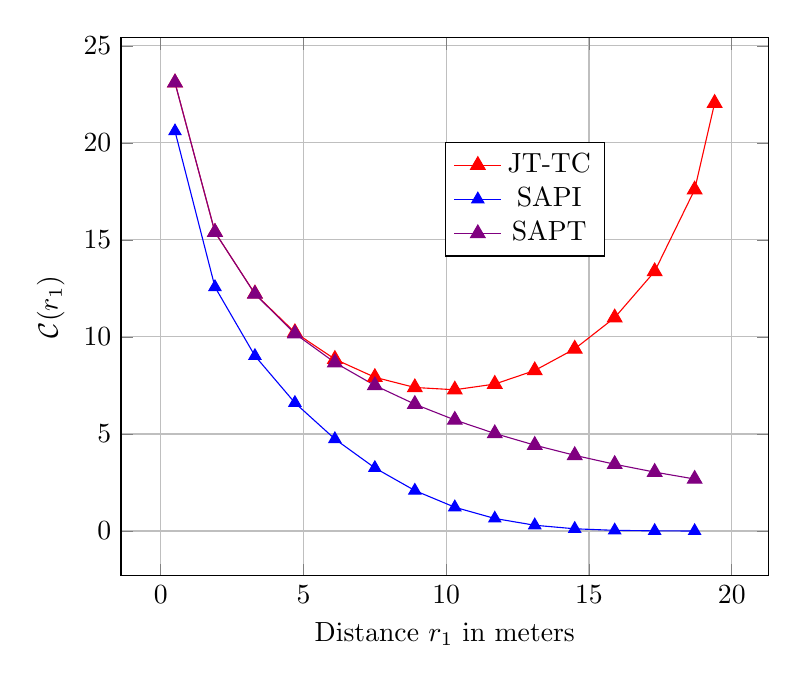
\begin{tikzpicture}
    	\begin{axis}[scale=1.2,
        	grid = both,
        	legend style={
        		at={(0.5,0.7)},
        		{anchor=west},
        		%cells={anchor=west},
        		%legend pos=north west,
        	},
        	xlabel ={Distance $r_1$ in meters},
        	ylabel = {$\mathcal{C}(r_1)$}
        	]
        	\addplot[mark=triangle*, mark size=3,color=red]
        	coordinates{
        		(0.500000, 23.098800) (1.900000, 15.396600) (3.300000, 12.224300) (4.700000, 10.232700) (6.100000, 8.853340) (7.500000, 7.920660) (8.900000, 7.394910) (10.300000, 7.277360) (11.700000, 7.570650) (13.100000, 8.269810) (14.500000, 9.384460) (15.900000, 10.993200) (17.300000, 13.373900) (18.700000, 17.585200) (19.400000, 22.046700) 
        	};\addlegendentry{$\mbox{JT-TC}$}
        	\addplot[mark =triangle*,  mark size=2.5, color=blue]
        	coordinates{
        		(0.500000, 20.600000) (1.900000, 12.570000) (3.300000, 9.023000) (4.700000, 6.604000) (6.100000, 4.738000) (7.500000, 3.250000) (8.900000, 2.084000) (10.300000, 1.224000) (11.700000, 0.644600) (13.100000, 0.296100) (14.500000, 0.113600) (15.900000, 0.033400) (17.300000, 0.006134) (18.700000, 0.000348) 
        	};\addlegendentry{$\mbox{SAPI}$}
        	\addplot[mark=triangle*, mark size=3, color=violet]
        	coordinates{
        		(0.500000, 23.100000) (1.900000, 15.400000) (3.300000, 12.210000) (4.700000, 10.170000) (6.100000, 8.678000) (7.500000, 7.500000) (8.900000, 6.534000) (10.300000, 5.721000) (11.700000, 5.025000) (13.100000, 4.423000) (14.500000, 3.899000) (15.900000, 3.439000) (17.300000, 3.034000) (18.700000, 2.678000) 
        	};\addlegendentry{$\mbox{SAPT}$}
        	
            %	\addplot[mark =square*,  mark size=1.5, dashed, color=blue]
            %	coordinates{
            %		(1.000000, 5.398940) (2.000000, 3.417900) (3.000000, 2.303690) (4.000000, 1.576860) (5.000000, 1.083230) (6.000000, 0.745714) (7.000000, 0.515673) (8.000000, 0.359448) (9.000000, 0.253382) (10.000000, 0.181075) (11.000000, 0.131382) (12.000000, 0.096845) (13.000000, 0.072522) (14.000000, 0.055144) (15.000000, 0.042543) (16.000000, 0.033270) (17.000000, 0.026348) (18.000000, 0.021111) (19.000000, 0.017098) 
            %	};\addlegendentry{$(\mbox{SAPT},35)$}
            %	
    	\end{axis}
	\end{tikzpicture}
	\caption[Average Achievable Rate]{Average achievable rate $\mathcal{C}$ in b/s/Hz plotted against distance from $AP_1$ of a user for transmit $\snr = 60$dB.}
	%NJT means conventional network without joint transmission.}
	\label{fig:rate_theory}
\end{figure}




\subsection{Achievable rates with MIMO-JT}
\label{subsec:MIMO-JT_rates}
Now we provide the analysis of achievable rates of Joint Transmission with MIMO systems. When APs equipped with $N_t$ antennas and users with $N_r$ antenna, the link level capacity is given by the well-established capacity formula of MIMO system given by \cite{Telatar_MIMO_cap,TseViswa_Funda}, 
\begin{align}\label{eqn:Shann_MIMO}
R = \E \left[ \log \det \left| \I_{N_r} + \frac{\gamma_t}{N_t} \H \H^* \right|\right], 
\end{align}
where $\gamma_t=P_t/\sigma^2$ is the transmit signal to noise ratio. It should be noted that the path loss is included in the channel matrix, $\H$. We assume coherent combining of channels in JT-MIMO, hence we can use $\H = \H_1 + \H_2$ in \eqref{eqn:Shann_MIMO} to obtain achievable rates, where $\H_1$ and $\H_2$ are channels seen by the user from $AP_1$ and $AP_2$.


\subsubsection{Achievable rates for ZF-DPC based precoding for MIMO-JT}
%\thispagestyle{empty}
When the channel state information is available at the transmitters, precoding techniques like dirty paper coding (DPC) can achieve the Shannon limits \cite{Costa_DPC}. Many suboptimal  algorithms with reduced complexity, like THP, ZF-DPC are also discussed in the literature for link-level MIMO and CoMP \cite{Erex_DPC, SpencerZFMU, HarashimaMiyakawa, Tomlinson}.  

When using a single transmitter, we perform ZF-DPC as  follows: 
We assume both APs and STA are having the same number of antennas $N_t=N_r=N$.
Let the channel matrix be $\H$ and transmit signal vector be $\Vec{x} = [x_1,x_2,\hdots, x_{N}]^T$. The signal $\Vec{x}$ will be precoded before transmission using $\W = \Q^H$, obtained by the $\Lb \Q$ decomposition of $\H$, \ie, $\H=\Lb \Q$. Hence the received vector can be given as,  
\begin{align}
    \Vec{y} &= \H \W \Vec{x}+ \Vec{n} = \Lb \Vec{x}+\Vec{n}.
    \label{eq:DF_DPC}
\end{align}
Let $l_{ij}$ be the element in the $i^{th}$ row and $j^{th}$ column of $\Lb$. The $i^{th}$ row of the received signal $\Vec{y}$ can be written as 
\begin{align*}
{y_i} &= {l_{ii} x_{i} + \sum_{j<i} l_{ij} x_j + n_i}.
\end{align*}
The precoder $\W$ cancels interference from streams with indices $j>i$. The remaining interference terms with indices $j<i$ are taken care of by applying DPC. Therefore, the post-processing $\snr$ for $i^{th}$ stream is given by
\begin{align}\label{eq:sinr-downlink}
\gamma_{i}=\frac{P|l_{ii}|^2}{\sigma^2},
\end{align}
and then the achievable rate on $i$th stream is given by
\begin{align}\label{eqn:per_stream_rate}
R_i = \log [ 1+\gamma_i],
\end{align}
so that the net achievable rate is 
\begin{align}\label{eqn:net_rate_gen}
R = \sum_{i} R_i.
\end{align}
When used under the JT-TC scheme, the THP approach is to be modified to take into account the LQ decomposition of the channel matrices seen by the receiver, i.e., the LQ decomposition is done for individual channels and precoded streams are sent, and combined at the receiver\footnote{We can see that $\H^{(i)}$ are uncorrelated with the independent Rayleigh assumption.}. Thus, the received signal can be written as,
\begin{align}
\y&=\sum_{k=1}^{L}\Lb^{(k)}\x+\No,
\label{eq:DF_DPC_adv}
\end{align}
where $\Lb^{(i)}$ is the LQ decomposition of channel $\H^{(i)}$ from $i$th AP.
Therefore in two AP coordination, $i$th stream will be having a $\snr$,
\begin{align}\label{eqn:SNR_JT_MIMO}
\gamma^{JTM}_i=\frac{P_1 |l^{(1)}_{ii}|^2+P_2 |l^{(2)}_{ii}|^2}{\sigma^2},
\end{align} 
where $l^{(k)}_{ij}$ is the element in the $i$th row and $j$th column of $\Lb^{(k)}$. 

\begin{theorem}\label{the:cap_MIMO_JT}
	The achievable rate of $N\times N$ MIMO with two AP JT-TC using ZF-DPC is given by
	\begin{align}
	\mathcal{C}^{JM}(r_1,r_2)&=\one(a\neq b)
	\sum_{i=1}^{N} \sum_{l=0}^{N-i} \left( \frac{{N-i \choose l}\left(-1\right)^l }{(b-a)^{N-i+1}((N-i)!)^2} 
	\int_{0}^{\infty}\frac{\log_2(1+z)\Lambda_{\beta}(z,l+N-i+1)l}{\beta^le^{z/b}z^{l-N+i}}\d z\right) \nonumber\\
	&+\one(a= b) \sum_{i=1}^{N} \sum_{l=0}^{N-i} \frac{(a^2)^{N-i}}{((N-i)!)^2}\frac{{N-i \choose l}(-1)^{l} \int_{0}^{\infty} \log_2(1+z)e^{-z/a}z(z^2)^{N-i} \d z}{2(N-i)-l+1}
	\end{align}
	where $a = P_1 r_1^{-\alpha} / \sigma^2$, $b=P_2 r_2^{-\alpha} / \sigma^2$ and $\Lambda_{\beta}(z,k)$ is defined in \eqref{eqn:Lambda_def}.
\end{theorem}
\begin{proof}
	Refer appendix \ref{proof:theorem-ber-jt-mimo}.
\end{proof}

The capacity for various configurations of $(N_t,N_r)$ are plotted in Figure~\ref{fig:rate_theory_mimo}. Here, $r_1 + r_2 = R$ and the STA is travelling in a straight line between the two APs. The capacity for SAPT with MIMO can be obtained by substituting $P_2=0$ in Theorem~\ref{the:cap_MIMO_JT}.  We can see the improvement of cell edge rate with JT as in the case of single antenna transmissions. 

\begin{figure}[!]
	\centering 
	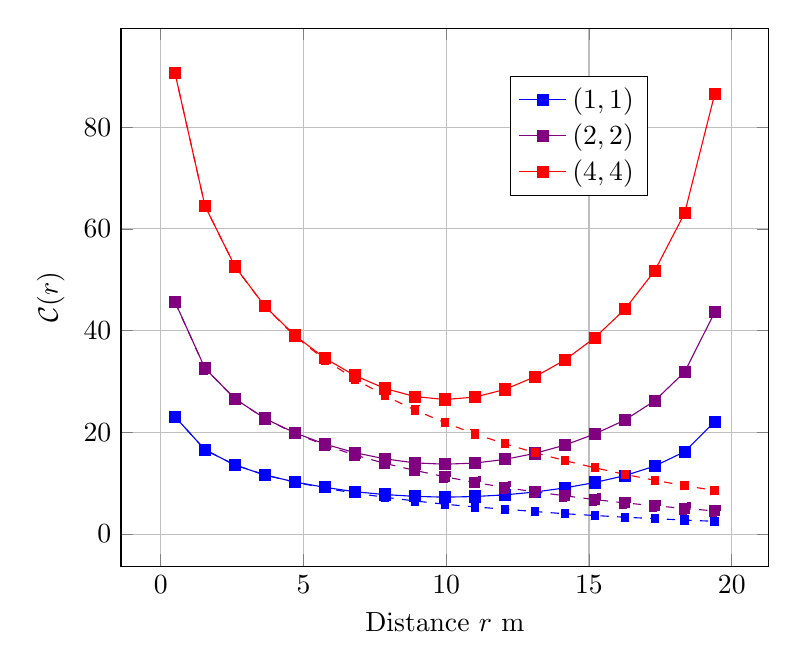
\begin{tikzpicture}
	\begin{axis}[scale=1.2,
	grid = both,
	legend style={
		at={(0.6,0.8)},
		{anchor=west},
		%cells={anchor=west},
		%legend pos=north west,
	},
	xlabel ={Distance $r$ m},
	ylabel = {$\mathcal{C}(r)$}
	]
%	\addplot[mark=triangle*, mark size=2,color=red]
	\addplot[mark =square*,  mark size=2, color=blue]
	coordinates{
		(0.500000, 23.084789) (1.550000, 16.570610) (2.600000, 13.566926) (3.650000, 11.618182) (4.700000, 10.234375) (5.750000, 9.192601) (6.800000, 8.326384) (7.850000, 7.773324) (8.900000, 7.411785) (9.950000, 7.257085) (11.000000, 7.384026) (12.050000, 7.710342) (13.100000, 8.259237) (14.150000, 9.072991) (15.200000, 10.134842) (16.250000, 11.485551) (17.300000, 13.359518) (18.350000, 16.201779) (19.400000, 22.067556) 
	};\addlegendentry{$(1,1)$}
	\addplot[mark =square*,  mark size=2, color=violet]
	coordinates{
		(0.500000, 45.652650) (1.550000, 32.595689) (2.600000, 26.623091) (3.650000, 22.708549) (4.700000, 19.898565) (5.750000, 17.692942) (6.800000, 16.010082) (7.850000, 14.789587) (8.900000, 13.996781) (9.950000, 13.737852) (11.000000, 13.957857) (12.050000, 14.680674) (13.100000, 15.856917) (14.150000, 17.493510) (15.200000, 19.669542) (16.250000, 22.397844) (17.300000, 26.198307) (18.350000, 31.873375) (19.400000, 43.585118) 
	};\addlegendentry{$(2,2)$}
	
%	\addplot[mark=triangle*, mark size=2,color=green]
%	coordinates{
%		(0.500000, 68.159654) (1.550000, 48.564703) (2.600000, 39.627644) (3.650000, 33.753238) (4.700000, 29.483754) (5.750000, 26.140879) (6.800000, 23.591430) (7.850000, 21.723103) (8.900000, 20.545081) (9.950000, 20.107264) (11.000000, 20.479619) (12.050000, 21.569081) (13.100000, 23.372341) (14.150000, 25.862381) (15.200000, 29.094360) (16.250000, 33.282926) (17.300000, 38.956277) (18.350000, 47.500747) (19.400000, 64.981016) 
%	};\addlegendentry{$(3,3)$}

	\addplot[mark =square*,  mark size=2, color=red]
	coordinates{
		(0.500000, 90.640776) (1.550000, 64.516821) (2.600000, 52.616732) (3.650000, 44.776224) (4.700000, 39.050575) (5.750000, 34.560896) (6.800000, 31.167549) (7.850000, 28.637729) (8.900000, 27.031495) (9.950000, 26.462736) (11.000000, 26.925780) (12.050000, 28.428948) (13.100000, 30.903238) (14.150000, 34.205860) (15.200000, 38.595804) (16.250000, 44.172731) (17.300000, 51.744374) (18.350000, 63.105301) (19.400000, 86.457358) 
	};\addlegendentry{$(4,4)$}
	\addplot[mark =square*,  mark size=1.5,dashed, color=red]
	coordinates{
		(0.500000, 90.640764) (1.550000, 64.515507) (2.600000, 52.608276) (3.650000, 44.740296) (4.700000, 38.933798) (5.750000, 34.259963) (6.800000, 30.490931) (7.850000, 27.216507) (8.900000, 24.390347) (9.950000, 21.915066) (11.000000, 19.679343) (12.050000, 17.776746) (13.100000, 16.016981) (14.150000, 14.452914) (15.200000, 13.039510) (16.250000, 11.745088) (17.300000, 10.582326) (18.350000, 9.508882) (19.400000, 8.584689) 
	};

	\addplot[mark =square*,  mark size=2,dashed, color=violet]
	coordinates{
		(0.500000, 45.623906) (1.550000, 32.555297) (2.600000, 26.578839) (3.650000, 22.698928) (4.700000, 19.798465) (5.750000, 17.492858) (6.800000, 15.545089) (7.850000, 13.898479) (8.900000, 12.527735) (9.950000, 11.270269) (11.000000, 10.166871) (12.050000, 9.165769) (13.100000, 8.304833) (14.150000, 7.527499) (15.200000, 6.785055) (16.250000, 6.132034) (17.300000, 5.573062) (18.350000, 5.032646) (19.400000, 4.564343) 
	};

	\addplot[mark =square*,  mark size=1.5, dashed, color=blue]
	coordinates{
		(0.500000, 23.078415) (1.550000, 16.589099) (2.600000, 13.595400) (3.650000, 11.629084) (4.700000, 10.204372) (5.750000, 9.037901) (6.800000, 8.045143) (7.850000, 7.242525) (8.900000, 6.514277) (9.950000, 5.871401) (11.000000, 5.343287) (12.050000, 4.890189) (13.100000, 4.437960) (14.150000, 3.998739) (15.200000, 3.654645) (16.250000, 3.315731) (17.300000, 3.037490) (18.350000, 2.754235) (19.400000, 2.504608) 
	};
	\end{axis}
	\end{tikzpicture}
	\caption[Average Achievable Rate]{Average rate $\mathcal{C}$ in b/s/Hz achievable for MIMO-JT-TC along with average rate from $AP_1$ Vs distance from $AP_1$ of a user for various combinations of $(N_t,N_r)$ at $\snr=60$ dB. The dashed curve corresponds to SAPT for the respective configurations.}% NJT means conventional network without joint transmission.}
	\label{fig:rate_theory_mimo}
\end{figure}


%third section
\section{A Network Scenario}
\label{sec:system_definition}
To incorporate a wider range of scenarios, we defined a new system model that is more generalized. This model can handle multiple APs with multiple channels available, and multiple STAs. This section describes the system model with capacity metric analysis and provides an example scenario.


% Defining the system in terms of channels and APs
\subsection{System Elements}
Let us say there are $N_{AP}$ APs and $N_{Ch}$ frequency channels available where each AP is assigned only one channel.
Now, there can be two scenarios:
If $N_{AP} \leq N_{Ch}$, we have enough channels for each AP and each can transmit on its own channel without causing interference for others.
If $N_{AP} > N_{Ch}$, we don't have enough channels for each AP and some of them will have to share channels.
This may result in interference and using Joint Transmission would be a feasible option. In this paper we will explicitly assume a system where $N_{AP} > N_{Ch}$.

The APs which will use the same channel to transmit to different users will cause interference to both the users. Such APs are also eligible for Joint transmission to a common user.
Let us define the interference sets $\I_i$ of APs who transmit in the same channels. These sets are given as
\begin{align*}
    & (AP_1^1,AP_2^1,AP_3^1,\ldots,AP_{F_1}^1) &&= \I_1,\\
    & (AP_1^2,AP_2^2,AP_3^2,\ldots,AP_{F_2}^2) &&= \I_2,\\
    & (AP_1^3,AP_2^3,AP_3^3,\ldots,AP_{F_3}^3) &&= \I_3,\\
    & \ldots&&\quad\vdots\\
    & (AP_1^i,AP_2^i,AP_3^i,\ldots,AP_{F_i}^i) &&= \I_i,\\
    & \ldots&&\quad\vdots\\
    & (AP_1^{N_{Ch}},AP_2^{N_{Ch}},AP_3^{N_{Ch}},\ldots,AP_{F_{N_{Ch}}}^{N_{Ch}})&& = \I_{N_{Ch}}.
\end{align*}
Here $AP_{j}^i \in \I_i$ is the j number of APs using the $i_{th}$ channel, and $F_i$ is the number of APs that use the same channel $i$. Also,
\begin{equation}
\label{eq:TotalAPs}
    \sum_{i=1}^{N_{Ch}} F_i = N_{AP},
\end{equation}
in other words, the sum of the number of APs in each set will be equal to the total number of APs in the system. That is, an AP is not allowed to hop channels.

All the APs in a set $\I_i$ will serve in the same channel and thus, if there are multiple APs in a set, Joint transmission can be utilized by these APs. 
In this paper, we will assume that the joint transmission does not happen across more than two APs, and also that only one pair of APs in channel $i$ can be involved in a joint transmission.
Without loss of generality, and for a simple notation, the above assumptions help us index the sets $\I_i$ in such a manner that
\begin{enumerate}
    \item Cardinality of $\I_i = 1$ or $F_i = 1, \: \forall \;i \leq N_{Ch}^*$, i.e., the APs in these sets will participate only in  SAPT,
    
    \item Cardinality of $\I_i = 2$ or $F_i = 2, \: \forall \;i > N_{Ch}^*$, i.e., the APs in these sets will participate both in Joint Transmission and SAPI (a particular set of AP either participate in Joint Transmission or in SAPI at any instant), 
\end{enumerate}
for some $N^*_{Ch}$ such that $N^*_{Ch}+2(N_{Ch}-N^*_{Ch}) = N_{AP}$. This also implies that the same AP cannot appear in multiple $I_i$, i.e., if an AP has been paired with another AP for JT, it cannot do JT with any other AP anytime.

For $a\in I_i, i\leq N_{Ch}^*$, the only possible mode of transmission is the SAPT mode. An AP $a\in I_i, i> N_{Ch}^*$ can serve an STA in either the SAPI mode or the JT mode (this is under the assumption that all the APs will always be transmitting, thus ruling out the possibility of SAPT transmission from such APs).





% Defining notations for different modes of transmission
\subsection{Scheduling Modes of STAs}
\label{subsec:schedulingModesOfSTAs}
For any STA, two scheduling methods are available, 
\begin{itemize}
    \item Joint Transmission (JT): This will only be possible for the APs that belongs to $\I_i$ for $i > N_{Ch}^*$.
    
    \item Non-JT: This would be possible using SAPT or SAPI, depending on whether the AP serving the STA belong to $\I_i$ for $i \leq N_{Ch}^*$, or $ > N_{Ch}^*$, respectively.
\end{itemize}

Assuming there are $N_S$ STAs in the system, each STA is located at some position in a 2D space.
For any $a \in I_i$, we have
$$S_a = \{\text{All the STAs getting served by AP } a \},$$
and
$$N_S(a) = \text{The number of STAs served by AP } a.$$
It will be assumed that the set $S_a$ is an ordered set and the $k^{th}$ element of this set will be denoted by $S_a(k)$.
% ^^^
% We will represent the STAs with $S_i$, where $i = 1, 2, \ldots, N_S$.
% \[
% S(x,y) = 
% \begin{cases}
%   \{a\} & \text{a $\in$ $\I_i$; \ i $\leq N_{Ch}$} \\
%   I_i & \text{for some $i<N_{Ch}^*$}
% \end{cases}
% \]

The set $S_a$ can be further divided into two sets; the STAs getting served using JT mode can be represented as $S^J$ where
\begin{equation*}
    S_a^J = \{\text{All the STAs getting served by AP } a \text{ using JT mode}\},
\end{equation*}
and the STAs getting served using Non-JT mode can be represented as $S^S$ where
\begin{equation*}
    S_a^S = \{\text{All the STAs getting served by AP } a \text{ using a non-JT mode}\}.
\end{equation*}

Similarly, we also have
\begin{equation*}
    N_S^J(a) = \text{The number of STAs served by AP } a \text{ using JT mode},
\end{equation*}
and
\begin{equation*}
    N_S^S(a) = \text{The number of STAs served by AP } a \text{ using a non-JT mode}.
\end{equation*}

In a given scenario, it is possible for an AP to serve different STAs in different modes, but an STA will be served using only one mode by the same APs.
In other words, we can have both $S_a^J$ and $S_a^S$ to be not NULL, \ie, $S_a^J, S_a^S \neq \Phi$, for some AP $a \in I_i, i > N_{ch}^*$ and $S_a^J$ and $S_a^S$ will always be mutually exclusive sets, \ie , $S_a^J\cap S_a^S = \Phi$. Also,
\begin{equation}
    N_S(a) = N_S^J(a) + N_S^S(a),
\end{equation}
and
\begin{equation}
    \label{eq:STAsumInDifferentModes}
    N_S = \sum_a N_S^S(a) + \frac{1}{2} \sum_a N_S^J(a).
\end{equation}

We are assuming that for a given scenario the locations of APs are fixed and STAs are stationary (does not change frequently), and thus the scheduling of the STAs would not change with time.

\subsection{Per-Slot Scheduling}
\label{subsec:perSlotScheduling}
We are assuming a Slotted Scheduling algorithm with the following properties:
\begin{itemize}
    \item \textit{Maximum Utilization:} All the APs will always transmit in every slot.
    
    \item \textit{Intra-AP Fairness:} All STAs in $S_a$ are served using a round-robin like approach by AP $a$ (For a particular AP, each user gets the same amount of time as other users getting served by the same AP. This does not imply that every user in the system is getting served for equal time).
    
    % \item All AP $a \in I_i, i > N_{Ch}^*$ will serve the same number of users.
    % Which means $N_S(a) = \text{Constant } \forall a \in I_i$.
    \item For two APs $a, b \in I_i, i > N_{Ch}^*$ with $S_a^J \cap S_b^J \neq \Phi$, it will be assumed that $N_S^S(a) = N_S^S(b)$ and $N_S^J(a) = N_S^J(b)$, implying $N_S(a) = N_S(b)$. Furthermore, $S_a^J = S_b^J$.
    
\end{itemize} 

Using the notation introduced in subsection \ref{subsec:schedulingModesOfSTAs}, we can provide a pictorial view of the round-robin-like scheduling.
% An AP $a\in \I_i$ for $i \leq N_{Ch}^*$ serves all its $N_S(a)=N_S^S(a)$ STAs from $S_a^S$ in a round-robin manner,  


\begin{figure}[h]
    \begin{center}
        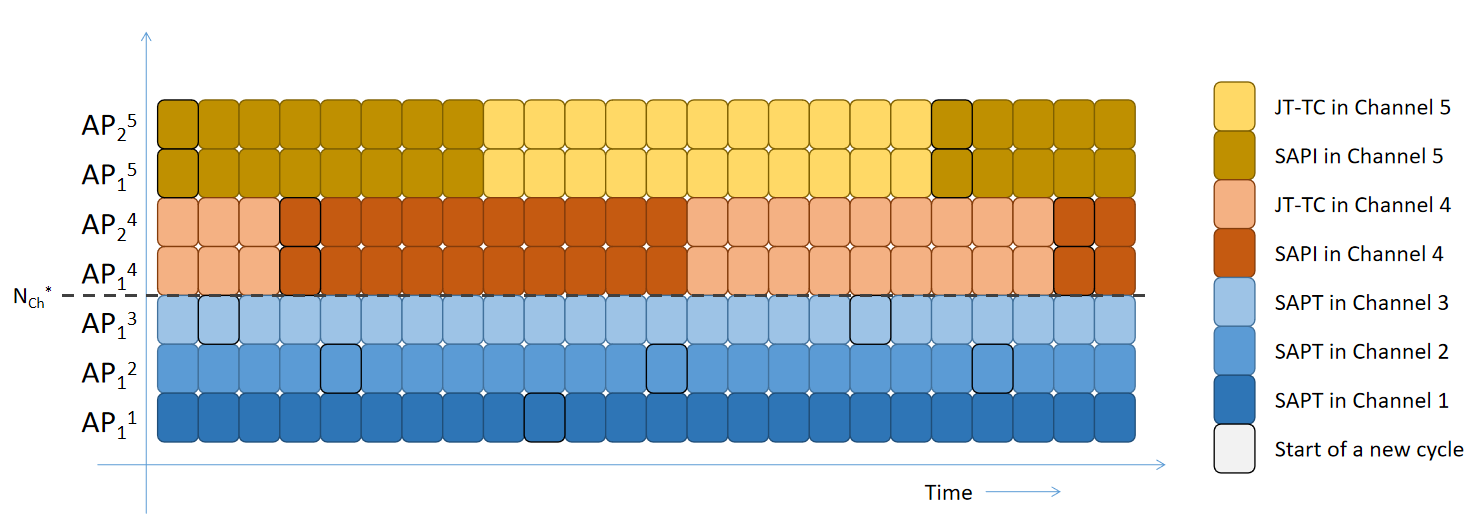
\includegraphics[width=6.5in]{Scheduling.png}
        \caption{A small interval of a scheduling timeline.}
        \label{fig:Scheduling}
    \end{center}
\end{figure}

%\begin{figure*}[h]
%	\centering
%	\begin{subfigure}[t]{0.75\linewidth}
%		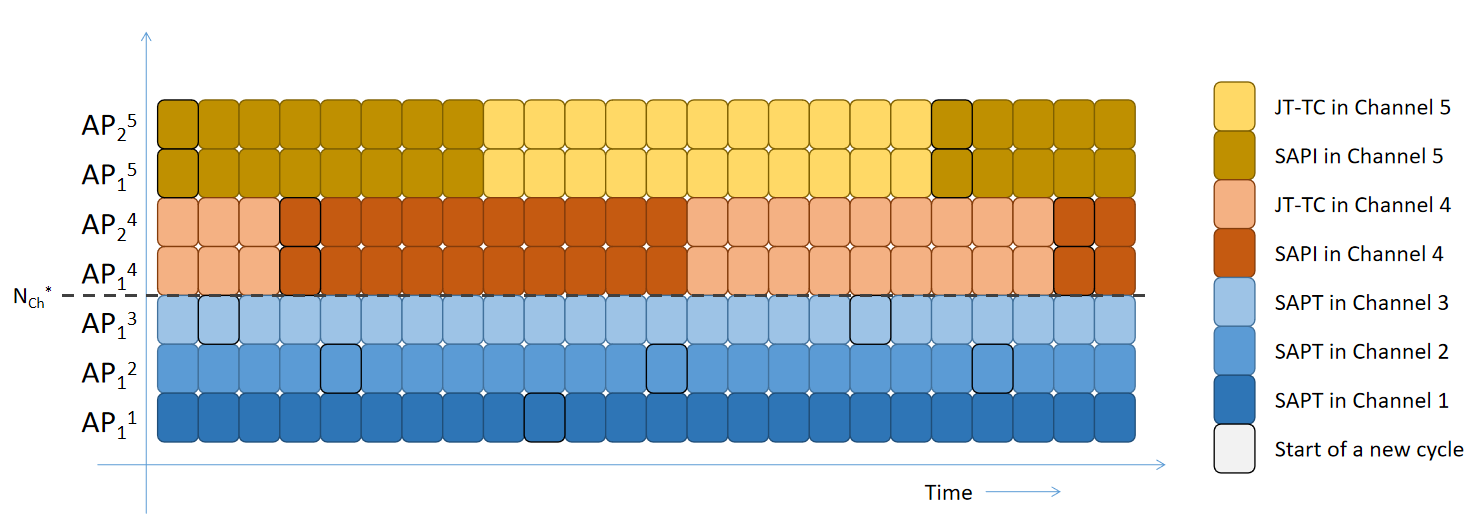
\includegraphics[width=\linewidth]{Scheduling.png}
%		%\caption{non-JT} %caption for sub figure 1
%       \label{fig:non-JT_scheduling}
%	\end{subfigure}
%	\begin{subfigure}[t]{0.2\linewidth}
%		\includegraphics[width=\linewidth]{legend.png}
%		%\caption{JT} %caption for sub figure 2
%        \label{fig:JT_scheduling}
%	\end{subfigure}
%	\caption[AP assignments]{A part of a scheduling timeline}
%	\label{fig:mimo_jt_edge}
%\end{figure*}


Figure~\ref{fig:Scheduling} shows what the above mentioned typical schedule will look like.
This figure only covers a part of the scheduling timeline. There can be different number of STAs assigned to APs with different modes in some set $\I$.
% of transmission and the STAs will not always be synchronized in order.
% , but with every AP assigned with the finite number of users, it will happen frequently that the STAs will align for the same time-slot.
% An AP  $a\in \I_i$ for $i > N_{Ch}^*$ serves all its $N_S^S(a)$ STAs from $S_a^S$ in a round-robin manner, and then serves the STAs from $S_a^J$ in round-robin manner again. Note that these STAs from $S_a^J$ are simultaneously served by $b\in \I_i$ such that $S_a^J=S_b^J$.






\subsection{Performance Under a Schedule}
\label{subsec:system_analysis}
%\subsection{System Inputs}
For any given STA, located at $(x,y)$, an offline capacity matrix is assumed to be available. Let's say we have given input,
\[C_a (x,y), \quad \forall \  a \in \bigcup\limits_{i=1}^{N_{Ch}} I_{i},\]
where $C_a(x, y)$ is the \textbf{Best Capacity} provided by the AP $a$ to an STA at the position $(x, y)$ in Non-JT mode, and
\[C_I (x,y), \quad \forall I = \{a,b\} \subseteq I_i, i > N_{Ch}^*,\]
where $C_I(x, y)$ is the \textbf{Best Capacity} provided by the Joint Transmission done by the APs in $I$ to an STA at the position $(x, y)$.
% If $a\in I_i, i>N^*_{Ch}$, then as per scheduling policy, all the APs in $I_i$ are transmitting at the same time (to same or different STAs).

Capacity of a user at $(x,y)$ with Joint Transmission is obtained by using Theorem~\ref{theo:rate_JT}, where $(x,y)$ is at distance $r_1$ from $a_1$ with transmit power $P_1$ and at $r_2$ from $a_2$ with transmit power $P_2$, and $a_1$, $a_2$ $\in$ $\I_i$
% is at distance $r_1$ from $a_1$ and $r_2$ from $a_2$ 
%\begin{align}\label{eqn:rate_jt_sch}
%	\mathcal{T}^{JT} (x,y)_{(r_1,r_2)} &=\frac{1}{\log
%		(2)}\frac{1}{P_1  r_1^{-\alpha}-P_2r_2^{-\alpha}}\nonumber\\ 
%	&\hspace*{-1cm}\times\left[P_1 r_1^{-\alpha } e^{\frac{\sigma ^2
%			r_1^{\alpha }}{P_1}} \Gamma
%	\left(0,\frac{\sigma ^2 r_1^{\alpha
%	}}{P_1}\right)\right.\nonumber\\
%&\left.-P_2 r_2^{-\alpha }
%	e^{\frac{\sigma ^2 r_2^{\alpha }}{P_2}}
%	\Gamma \left(0,\frac{\sigma ^2 r_2^{\alpha
%	}}{P_2}\right)\right]
%\end{align}
%	where $\Gamma(a,x)$ is the incomplete gamma function\footnote{$\Gamma(a,x)=\int_{x}^{\infty} t^{a-1}e^{-t}\d t$}.
	
%Here (x,y) is at distance $r_1$ from $a_1$ with transmit power $P_1$ and  at $r_2$ from $a_2$ with transmit power $P_2$, where $a_1$, $a_2$ $\in$ $\I_i$

%SAPI
Capacity of a user at $(x,y)$ with SAPI is obtained by using Theorem~\ref{Theo:SAP_with_interf}, where $(x,y)$ is at distance $r_1$ from $a_1$ with transmit power $P_1$ and at $r_2$ from $a_2$ (uncoordinated AP) which interfere with transmit power $P_2$, and $a_1, a_2 \in \I_i$.

%\begin{align}\label{eqn:SAPI_rate_sch}
%	\mathcal{T}^{SAPI} (x,y)_{(r_1,r_2)} &=\int_{0}^{\infty}\frac{e^{-\sigma^2(2^t-1)/P_1r_1^{-\alpha}}}{1+(2^t-1)\frac{P_2r_2^{-\alpha}}{P_1 r_1^{-\alpha}}}\d t.
%	\end{align}

%Here (x,y) is at distance $r_1$ from $a_1$ with transmit power $P_1$ and at $r_2$ from $a_2$ (uncoordinated AP) interfere with transmit power $P_2$, where $a_1$, $a_2$ $\in$ $\I_i$\\

%SAPT

%Capacity of a user at (x,y) with SAPT is given by using corollary 2 
% \begin{align}
%	\mathcal{T}_a^{SAPT}(x,y)_r&=\frac{e^{\frac{\sigma ^2 r^{\alpha }}{P}} \Gamma
%		\left(0,\frac{r^{\alpha } \sigma ^2}{P}\right)}{\log
%		(2)}
%	\end{align}
 
 %Here (x,y) is at distance r from an AP a which is transmitting with power P, where a $\in$ $\I_i$ \\
 %Scheduling:
 
 
 

For making the system's performance better, first, we need a way to analyse the system.
For a given schedule, we start with calculating the average throughput that an AP can provide to all of its STAs in different modes.
The average capacity for all the STA provided by the AP will be simply the average of Capacities of all the STAs by that AP.
We will calculate the Capacities of different modes of transmission separately. It will allow us to compare the benefits of these modes.

For a system, let $S_a^S(n)$ be the $n^{th}$ STA getting served in a non-JT mode and $S_a^J(n)$ be the $n^{th}$ STA getting served in a JT mode by the AP $a$.
Then, the Average capacity of the AP $a$ serving in non-JT mode will be given as
\begin{equation}
    C_{AP}^S(a) = \frac{1}{N_S^S(a)} \times \sum_{n=1}^{N_S^S(a)} C_a(S_a^S(n)).
\end{equation}
And, the Average capacity of all the APs $a \in I$ serving in JT mode will be given as
\begin{equation}
    C_{AP}^J(I) = \frac{1}{N_S^J(a)} \times \sum_{n=1}^{N_S^J(a)} C_I(S_a^J(n)).
\end{equation}
The above equations are based on the assumption of intra-ap fairness, i.e., every STA assigned for that AP is served for the same amount of time.

As one AP will be serving multiple STAs and possibly in different transmission modes, an STA will only receive a fraction of the resource.
If the total time to serve all the assigned STAs is $T$, then each STA is being served for $T / N_S(a)$ time.
This means the average capacity received by the user from an AP $a$ using non-JT mode will become the total bits received by the User per Hz divided by the total time,
\begin{align} %avgCapacityForUser(i)
    \label{eq:avgCapacityForUserNJT}
    C_{User}^a &= \frac{1}{T} \times \frac{T}{N_S(a)} \times C_{AP}^S(a) \nonumber
    \\
    &= \frac{1}{N_S(a)} \times C_{AP}^S(a).
\end{align}
Similarly, for all the users getting served by AP $a \in I$ using non-JT mode, and
\begin{equation} %avgCapacityForUser(i)
    \label{eq:avgCapacityForUserJT}
    C_{User}^I = \frac{1}{N_S(a)} \times C_{AP}^J(I).
\end{equation}

At any given instance, the net Capacity/throughput that the system will be providing will be the sum of the capacities being received by all the users at that instance.
For a long time average, this Capacity will become the sum of the average capacity the users served by all the APs in different modes.
Thus the total average capacity for the system will become,
\begin{equation}
    C_{Sys} = \sum_{i = 1}^{N_{Ch}^*} \sum_{a \in I_i} C_{User}^a +
    \left( 
    \sum_{i = N_{Ch}^* + 1}^{N_{Ch}} \sum_{a \in I_i} C_{User}^a  + 
    \sum_{i = N_{Ch}^* + 1}^{N_{Ch}} C_{User}^{I_i} 
    \right).
\end{equation}
Using eq. \ref{eq:TotalAPs}, We can simplify the above equation as
\begin{equation}
    C_{Sys} = \sum_{a=1}^{N_{AP}} C_{User}^a + 
    \sum_{i = N_{Ch}^* + 1}^{N_{Ch}} C_{User}^{I_i}.
\end{equation}

% \textcolor{red}{need to provide a general mathematical description of the system model.}







\subsection {An Example Scenario}
\label{subsec:an_example_scenario}
\label{example_scenario}
Consider an example scenario with 4 APs and 3 channels. Figure~\ref{fig:setup} shows a typical conference room deployment which is covered by $4$ access points installed at $4$ corners of the room. We have the three different channel sets $I_1$, $I_2$, and $I_3$ that are given as
\begin{align*}
    I_1 &= \{AP_1^1\},
    \\
    I_2 &= \{AP_1^2\},
    \\
    I_3 &= \{AP_1^3, AP_2^3\}.
\end{align*}
In this example, $N_{Ch}^* = 2$, i.e., APs in $I_1$ and $I_2$ are only capable of doing SAPT whereas APs in set $I_3$ are capable of doing both SAPI and JT-TC. The APs are installed at the corners of the room in the order $AP_1^1, AP_1^3, AP_1^2, AP_2^3$, such that the APs serving in the same channel are in the opposite corners of the room. The APs in the figure are color-coded according to the Channel they are serving in. The APs that are serving on the common channel frequency, i.e., APs $\in I_3$ are color-coded blue and the other APs that are serving on different channel frequency, i.e., APs $\in I_1$ and $I_2$ are using orange and yellow color respectively.

We considered that there are $N_S = 64$ STAs distributed uniformly in the square room. We already have the capacity values available %according to the above mentioned equations
from the simulation done in~\cite{JT_decision}. The tiles on the floor represent the association of end-users (STA located at that position, say a person sitting on a chair) to the different APs. These tiles are also color-coded according to the mode of transmission they are assigned to.
The Pink STAs represent the users that are served using Joint Transmission from the two blue APs (bottom-left and top-right corners), the blue tiles are served in SAPI manner by the nearest blue APs, while others tile colors represent SAPT from their nearest APs.
% A Deployment Scenario figure
\begin{figure}[h]
    \begin{center}
        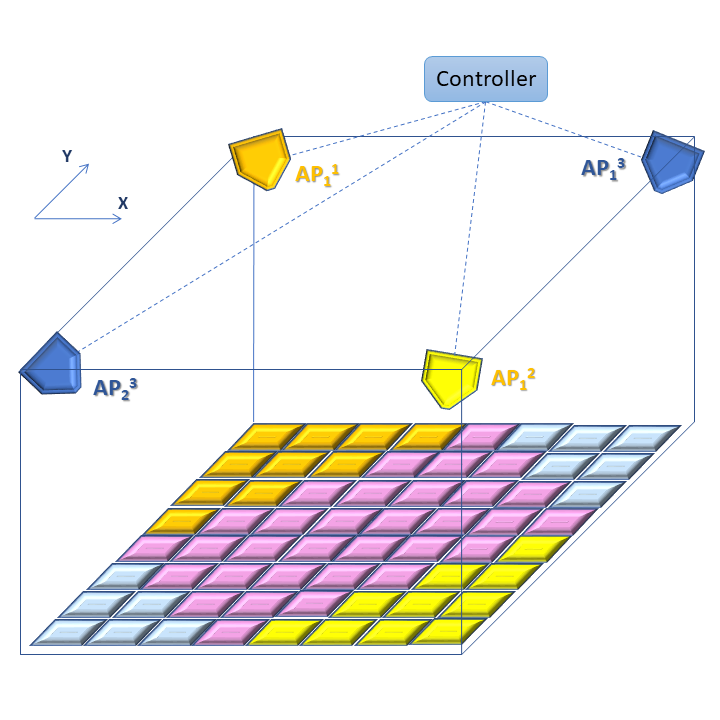
\includegraphics[scale=0.4]{Scenario.png}
        \caption{A deployment scenario.}
        \label{fig:setup}
    \end{center}
\end{figure}


%\textcolor{red}{ The System takes $N_S^S(a)$ and $N_S^S(a)$ (number of STAs each AP is serving in different modes) as an input and generate the Scheduling, assigning the APs with STAs that can receive higher throughput from it.}






\subsection{A Naive Scheduling Algorithm / Best transmission mode per User}
\label{subsec:naive_scheduling}
%\textcolor{red} {Consider the deployment scenario depicted in Figure~\ref{fig:setup}. The figure shows a typical conference room deployment which is covered by $4$ access points installed at the $4$ corners of the hall. Two $AP$s (color coded blue), $AP_a^i$ and $AP_b^i$ are assumed to be using the same center frequency (WiFi Channel) for operation, i.e., $AP_2$ and $AP_4 \in I_i$, $i>N_{ch}^*$  and the other $AP$s are using different channels, i.e., $AP_1$ and $AP_3 \in I_i$, i$<N_{ch}^*$. The colored tiles on the grids on the floor represent the association of end-users (located at that tile, say a chair) to the different $AP$s. The Pink tiles represent the users that are served using JT-TC from the two blue APs (bottom-left and top-right corners), other tile colors represent SAPT from their nearest $AP$s. The blue tiles on the grid are served in a SAPI manner by the nearest blue AP.} 

%\textcolor{red}{\emph{The decision problem is that of finding out which users should be served using JT-TC, SAPT and SAPI so that the total system throughput is maximized}. Note that we cannot have JT-TC using any other combination of APs as the orange and yellow APs are operating at different frequencies.} 

% A Deployment Scenario figure
%\begin{figure}[h ]
%\begin{center}
%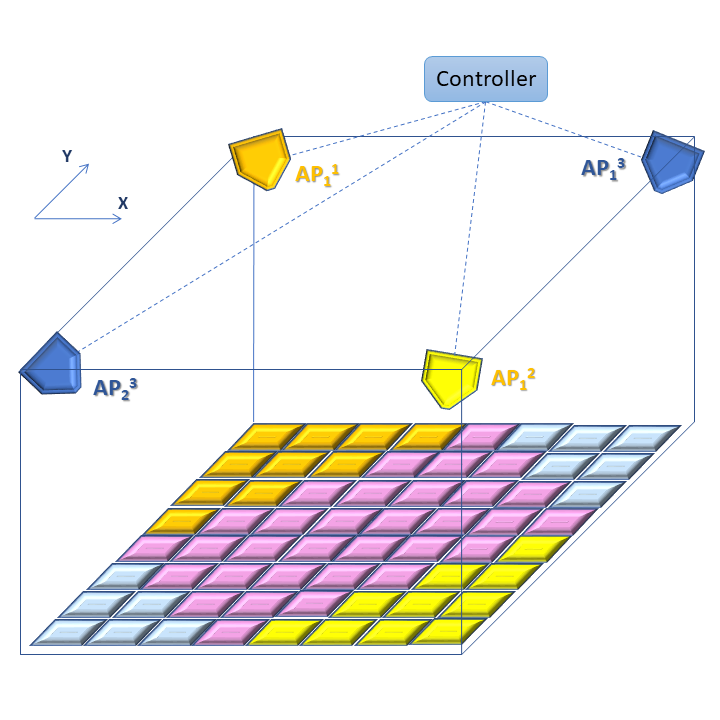
\includegraphics[width=3in]{Scenario.jpeg}
%\caption{A deployment scenario.}
%\label{fig:setup}
%\end{center}
%\end{figure}

In the above example, we will assume a symmetric scheduling mechanism, i.e., for $AP_1^3$ and $AP_2^3$ using the same frequency, we will compare for the blue and pink tiles using the following scheduling decisions:
\[{{Sched1}}:\ \ \ S(x,y) = \{AP_1^3\}, S(y,x) = \{AP_2^3\},\]
%\[{{Sched1}}:\ \ \ S(x,y) = \{AP_2^3\}, S(y,x) = \{AP_4\},\]
\ie, \emph{SAPI} to the tiles at locations $(x,y)$ and $(y,x)$, against
\[{Sched2}:\ \ \ S(x,y)=S(y,x)=\{AP_1^3, AP_2^3\},\]
i.e., Joint Transmission to the tiles at locations $(x,y)$ and $(y,x)$.
Here, S(x,y) is the set of APs used for transmission to the user/STA at location $(x,y)$, the set $\{ S(x,y) \}$ represent the scheduling decision.
Note that the ${Sched2}$ requires two time slots from the two APs to serve two different users, while ${Sched1}$ requires only one time slot to serve two users.
The symmetry assumption in $Sched1$ will be relaxed in section VI of this paper. The scheduling decision now reduces to the problem of determining whether
\begin{equation*}
    \label{eq:celledge_sym}
    C_{a}(x,y) + C_{b}(y,x) \geq C_I(x,y), \quad \forall \  I=\{a,b\} \subseteq I_i, i > N_{Ch}^*, %, s.t. S_{a}^J=S_{b}^J 
\end{equation*}
or due to symmetry we can say that,
\begin{equation}
    \label{eq:celledge}
    2 \ C_{a}(x,y) \geq C_I(x,y), \quad \forall \  I=\{a,b\} \subseteq I_i, i > N_{Ch}^*.  %, s.t. S_{a}^J=S_{b}^J 
\end{equation}

%\[2R_1(x,y) \geq R_2(x,y),\]
%where $R_i(x,y)$ is the rate received by the user at $(x,y)$ under scheduling rule $Schedi$.
%\thispagestyle{empty}
%When calculating, we see that for some specific conditions we can get a better rate when using 2AP uncoordinated transmission instead of JT-TC in the given symmetric condition.

To understand the relative values of the capacity achieved under $Sched1$ and $Sched2$, we considered a setup where two APs are situated $20$ meters apart and two STA are located at a distance $0\leq d \leq 10$ from the two APs (transmitting on the same frequency). The throughput obtained under joint transmission ($Sched2$) is compared with the sum of the throughput obtained by individual STAs under single AP transmission ($Sched1$). Figure~\ref{fig:threshold} provides the comparison for an individual AP transmit SNR of $101dB$ (corresponding to transmit power of $0dBm$ for a $20MHz$ bandwidth) and shows clearly that it is better to use $Sched1$ when $d<4.5m$ and use $Sched2$ when $4.5< d < 10$. Clearly, the exact threshold where this crossover happens will depend on the transmit SNR, the distance between the APs and the statistical characteristics of the channel used. 

\begin{figure}[h]
	\centering 
	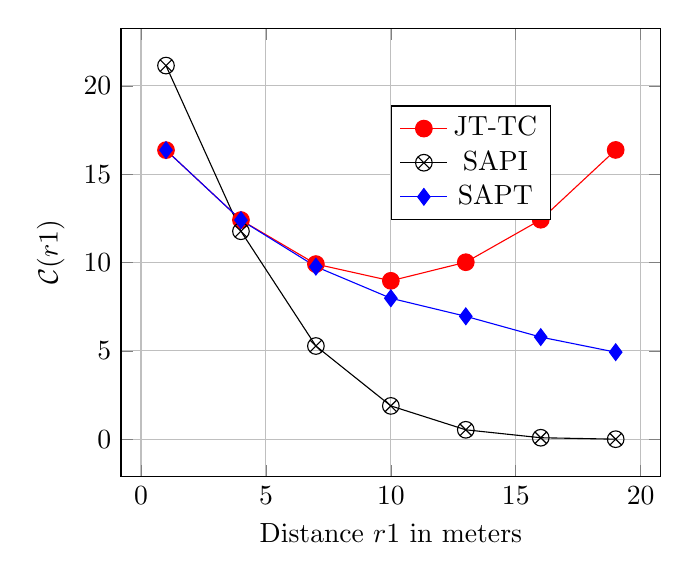
\begin{tikzpicture}
    	\begin{axis}[scale=1,
        	grid = both,
        	legend style={
        		at={(0.5,0.7)},
        		{anchor=west},
        		%cells={anchor=west},
        		%legend pos=north west,
        	},
        	xlabel ={Distance $r1$ in meters},
        	ylabel = {$\mathcal{C}(r1)$}
    	]
        	\addplot[mark=*, mark size=3,color=red]
        	coordinates{
        		(1.000000, 16.364038) (4.000000, 12.406548) (7.000000, 9.913230) (10.000000, 8.966414) (13.000000, 10.019064) (16.000000, 12.423531) (19.000000, 16.374288) 
        	};\addlegendentry{$\mbox{JT-TC}$}
        	\addplot[mark=otimes,  mark size=3, color=black]
        	coordinates{
        		(1.000000, 21.149659) (4.000000, 11.772189) (7.000000, 5.275936) (10.000000, 1.885351) (13.000000, 0.532592) (16.000000, 0.083208) (19.000000, 0.001724) 
        	};\addlegendentry{$\mbox{SAPI}$}
        	\addplot[mark=diamond*, mark size=3, color=blue]
        	coordinates{
        		(1.000000, 16.366059) (4.000000, 12.402396) (7.000000, 9.767942) (10.000000, 7.979081) (13.000000, 6.956606) (16.000000, 5.781152) (19.000000, 4.926368) 
        	};\addlegendentry{$\mbox{SAPT}$}
        	
    	\end{axis}
	\end{tikzpicture}
	
	\caption{Figure showing the crossover points for location where Joint transmission should be utilized when transmit $\snr=100$ dB. The crossover points of JT and SAPI can be seen to be 4 meters from $AP_1$.}
	\label{fig:threshold}
\end{figure}


%\textcolor{red}{ We have evaluated these scheduling schemes with extensive Monte-Carlo simulations. Matlab WLAN toolbox provides some pre-defined functions to simulate AP, STA, and the Wi-Fi channel using the IEEE 802.11 documents, \cite{matlab_wlan_toolbox}. We created transmission channels for each antenna element pair using the TGAC channel object and enabled path loss, \cite{brett_TGAC}. We passed the data signal through the channel and added Gaussian noise of fixed power and received them in their respected receiver antenna. The signals at the receiver were then combined using the MRC scheme (joint-transmission). Then we calculated the BER for different positions of the user between the two APs and plotted it in a graph.} %\st{Details of simulations using TGAC channel \cite{brett_TGAC} can be added here. Also we should emphasie the simulation of practical scenario is done.}
%\begin{figure}[h]
%\begin{center}
%\includegraphics[width=3in]{102.PNG}
%\caption{Figure showing the crossover points for location where Joint transmission should be utilized.}
%\label{fig:threshold}
%\end{center}
%\end{figure}



%\begin{figure}[h]
%	\centering 
%	\begin{tikzpicture}
%	\begin{axis}[scale=0.9,
%	grid = both,
%	legend style={
%		at={(0.5,0.7)},
%		{anchor=west},
%		%cells={anchor=west},
%		%legend pos=north west,
%	},
%	xlabel ={Distance $r$ from $AP_1$ in meters},
%	ylabel = {$\mathcal{C}(r)$}
%	]
%	\addplot[mark=triangle*, mark size=3,color=red]
%	coordinates{
%		(0.500000, 23.098800) (1.550000, 16.570500) (2.600000, 13.590700) (3.650000, 11.650300) (4.700000, 10.232700) (5.750000, 9.152950) (6.800000, 8.335290) (7.850000, 7.751310) (8.900000, 7.394910) (9.950000, 7.268170) (11.000000, 7.372900) (12.050000, 7.707560) (13.100000, 8.269810) (14.150000, 9.064480) (15.200000, 10.117000) (16.250000, 11.497000) (17.300000, 13.373900) (18.350000, 16.210000) (19.400000, 22.046700) 
%	};\addlegendentry{$\mbox{JT-TC}$}
%	\addplot[mark =triangle*,  mark size=2.5, color=blue]
%	coordinates{
%		(0.500000, 41.200000) (1.550000, 27.660000) (2.600000, 21.160000) (3.650000, 16.694000) (4.700000, 13.208000) (5.750000, 10.332000) (6.800000, 7.904000) (7.850000, 5.858000) (8.900000, 4.168000) (9.950000, 2.824000) (11.000000, 1.804000) (12.050000, 1.076400) (13.100000, 0.592200) (14.150000, 0.294600) (15.200000, 0.128400) (16.250000, 0.046300) (17.300000, 0.012268) (18.350000, 0.001758) (19.400000, 0.000036) 
%	};\addlegendentry{$\mbox{SAPI}$}
%	\addplot[mark=triangle*, mark size=3, color=violet]
%	coordinates{
%		(0.500000, 23.100000) (1.550000, 16.570000) (2.600000, 13.590000) (3.650000, 11.630000) (4.700000, 10.170000) (5.750000, 9.016000) (6.800000, 8.057000) (7.850000, 7.241000) (8.900000, 6.534000) (9.950000, 5.912000) (11.000000, 5.360000) (12.050000, 4.867000) (13.100000, 4.423000) (14.150000, 4.023000) (15.200000, 3.661000) (16.250000, 3.333000) (17.300000, 3.034000) (18.350000, 2.763000) (19.400000, 2.517000) 
%	};\addlegendentry{$\mbox{SAPT}$}
%
%	\end{axis}
%	\end{tikzpicture}
%	\caption[Average Achievable Rate]{Average achievable rate $\mathcal{C}$ in b/s/Hz Vs distance from $AP_1$ of a user for various values of $\snr=60$dB. The cross over points of JT and SAPI can be seen to be 6.45 meters from $AP_1$. \textcolor{red}{To be removed and just for a comparison.}}
%	%NJT means conventional network without joint transmission.}
%	\label{fig:rate_theory_jt_sapi_compa}
%\end{figure}
%
%



Figure~\ref{fig:threshold_2d} shows the impact of using such criteria on the scheduling in the two-dimensional grid of Figure~\ref{fig:setup} and marks the locations where joint transmission by $AP_1^3$ and $AP_2^3$ yields better throughput. The blue, pink and green tiles are showing two numerical values corresponding to the channel rates for JT-TC and SAPI assumptions, i.e., $Sched2$ and $Sched1$.
The tiles for which \eqref{eq:celledge} is satisfied are colored blue (SAPI), else colored pink. The green tiles are the ones where there is not much difference in JT-TC and SAPI. Orange and Yellow tiles are showing the corresponding SAPT rates.
%\textcolor{red}{This observation can be extended to a more general scenario in further sections}
%
\begin{figure}[h]
    \begin{center}
        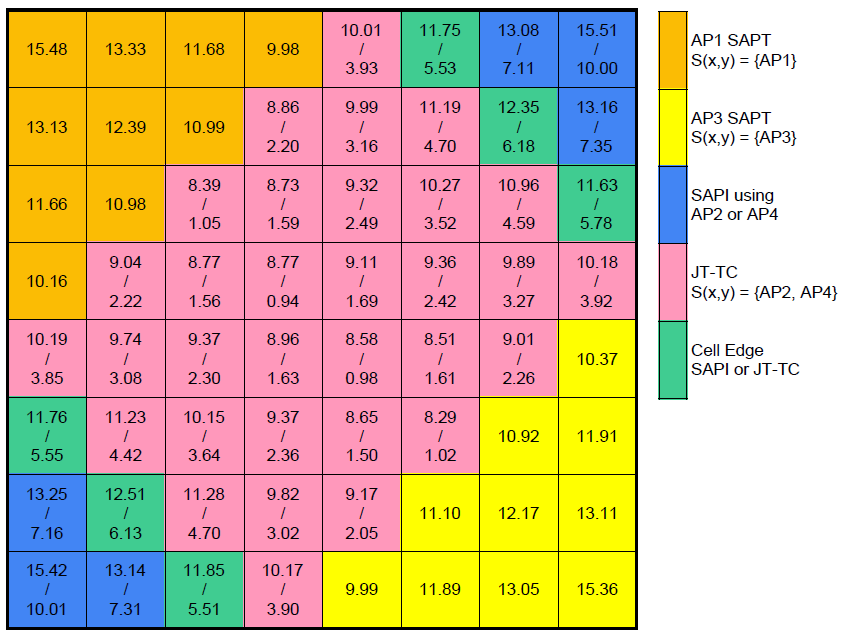
\includegraphics[width=4in]{data1_edited.png}
        \caption{Figure showing the crossover points for the location where Joint transmission should be utilized.}
        \label{fig:threshold_2d}
    \end{center}
\end{figure}

%\begin{figure}[h]
%\begin{center}
%\includegraphics[width=3in]{53.PNG}
%\caption{Figure showing the crossover points for location where Joint transmission should be utilized.\textcolor{red}{Explanation is missing!}}
%\label{fig:threshold_2d}
%\end{center}
%\end{figure}

\noindent\emph{Definition of Cell Edge:} As is clear from the observations of this section, we can refer to the STAs in the region \emph{just} qualifying for joint transmission (as per \eqref{eq:celledge}) as the cell edge devices in the context of IEEE 802.11be.

%\section{Considerations around transmit power}


\section{Online Scheduling for Maximising System level throughput}
\label{sec:optimal_scheduling}
% The scheduling policy described in the previous section works fine when only one user is needed to be served at once. But it doesn't consider the timing constraints that the system will have when serving multiple STAs simultaneously. 

The Algorithm discussed in the previous section is based on individual user perspective and is greedy in nature, and may lead to lower system level throughput because $N_S(a)$ may be high for some AP $a$ according to \eqref{eq:avgCapacityForUserNJT} and \eqref{eq:avgCapacityForUserJT} as per the schedule described in Figure~\ref{fig:Scheduling}.
In this section, we propose another scheduling policy that also takes account of the timing constraints, and develops an algorithm to provide a scheduling strategy to get better throughput for the system.

% To find the Optimal throughput achievable in the system, we used a reinforcement learning like approach.
% The approach consists of generating the system using some parameters as input. The system produces a performance value as its output. We alter one input parameter that improves the system performance until the performance cannot be further improved. The resulting system generated would have the best possible schedule for the system.




% We define the system with the number of channels available, the APs each channel has, with its locations, and the Number of STAs each AP will serve.
% The locations of APs and STAs are considered fixed and it is assumed that we already have all the Capacity values for every STA from each AP in all the modes available for the AP.

% We assign the STAs/tiles to each AP according to the maximum capacities each STAs can receive.
% Each AP will choose which STA it will serve according to the given average capacities.
% We calculate the maximum capacities the AP can provide and choose those STAs.
% %This ensures each vector N will generate a unique assignment of APs.

% Once every tile has been assigned to an AP, we can analyse the system for the total throughput being provided. To evaluate the system performance, we came up with the following criteria.

% In this section, we will discuss in detail about the inputs, outputs and their comparison along with a fairness criteria for a given system.




% \subsection{Criteria for optimal scheduling}
% \label{subsec:criteriaForOptimalScheduling}
Maximizing the throughput is one criterion to be considered. But having just this as a constraint can lead us to trivial solutions where only some users who have better capacity are getting served often while others starve. It gives us a very high system throughput but is not fair to the users. To impose some level of system fairness we came up with these two fairness criteria.

\subsubsection{Intra-AP fairness}
In subsection \ref{subsec:perSlotScheduling}, we already defined an assumption that the users will be served in a round-robin fashion for the equal time duration.
They are being served for the same amount of time and thus the STAs will get similar throughput from the AP according to the distance between them. This provides fairness among the STAs getting served by the same AP.

\subsubsection{Inter-AP fairness with mean/(standard deviation) like metric}
There is still a possibility that one AP may serve a very less number of STAs and thus provide higher average throughput to them compared to the AP which is serving a lot of STAs, and this is not ideal. To solve this problem, we compare the average throughput for the STAs served in different modes and try to reduce the variance among these values. The variance of the user capacities in the system can be calculated as
\begin{equation}
    \sigma_{C_{User}}^2 = var \left( \left( \bigcup\limits_{i = 1}^{N_{AP}} \big\{ C_{User}^{a_i} \big\} \right) \bigcup \left(
    \bigcup\limits_{i = N_{Ch}^* + 1}^{N_{Ch}} \big\{ C_{User}^{I_i} \big\} \right) \right)
\end{equation}

The ideal condition would be to reduce the value of $\sigma_{C_{User}}^2$ so that every STA gets fair throughput from all the APs.

We applied these criteria to a reinforcement learning algorithm to find a scheduling strategy that can provide high throughput to all users while maintaining fairness among them.
A pseudo code is provided in \textit{Algorithm \ref{algo:SchedulingAlgorithmPsudoCode}} that follows the above approach. A more detailed explanation about the inputs, system generation, outputs, and their comparison along with fairness criteria for this algorithm is provided below.




%[initialization]
%
%[assigning the APs]
%
%[iterating and refining the systems output]
\begin{algorithm}[h]
    \caption{Scheduling Algorithm}
    \label{algo:SchedulingAlgorithmPsudoCode}
    \begin{algorithmic}[1]
        \State Initialize $I_i$
        \State Input the values of $C_a$ and $C_I$, $\forall a \in \bigcup\limits_{i=1}^{N_{Ch}} I_{i}$ and $I=\{a,b\} \subseteq I_i, i > N_{Ch}^*, s.t. S_a^J=S_b^J$
        \State Initialize $\Vec{N}$
        \State Assign STAs to each AP according to $\vec{N}$ using \textbf{Algorithm \ref{algo:APAssignmentPsudoCode}}
        \State Calculate $C_{Sys}(\vec{N})$ and $\sigma^2_{C_{User}}(\vec{N})$
        \State Calculate the $P(\vec{N})$ as $C_{Sys}(\vec{N}) / \sigma^2_{C_{User}}(\vec{N})$
        \State Calculate the set $\Delta {N}$
        \While {System is not converged}
            \For {Every $\overrightarrow{\Delta n}$ in $\Delta{N}$}
                \State $\overrightarrow{newN} \gets \vec{N} + \overrightarrow{\Delta n}$
                \State Assign STAs to each AP according to $\overrightarrow{newN}$ using \textbf{Algorithm \ref{algo:APAssignmentPsudoCode}}
                \State Calculate $C_{Sys}(\overrightarrow{newN})$, and $\sigma^2_{C_{User}}(\overrightarrow{newN})$
                \State Calculate the P($\overrightarrow{newN}$) as $newC_{Sys}(\overrightarrow{newN}) / new\sigma^2_{C_{User}}(\overrightarrow{newN})$
                % \If {$performance>max-performance$}
                %     \State $max-performance \gets performance$
                %     \State $max-id \gets i$
                % \EndIf
                % \State calculate the change in $P(\vec{N})$ for $\vec{N}$ and $new\vec{N}$
            \EndFor
            \If {$(P(\vec{N}) - P(\overrightarrow{newN})) < 0, \forall \overrightarrow{newN}$}
                \State System converged, exit the while loop
            \Else
                \State $\vec{N} \gets \overrightarrow{newN}$ for the maximum $(P(\vec{N}) - P(\overrightarrow{newN}))$
                \State Assign STAs to each AP according to $\vec{N}$ using \textbf{Algorithm \ref{algo:APAssignmentPsudoCode}}
                % \State analyse the system for $\vec{N}$ and calculate $C_{Sys}$, $C_{User}^a$, $C_{AP}^a$, and $\sigma^2_{C_{User}}$
                % \State calculate the P($\vec{N}$) as $C_{Sys} / \sigma_{C_{User}}^2$
            \EndIf
        \EndWhile
    \end{algorithmic}
\end{algorithm}



% \subsection{Discussing the algorithm}
\subsection{Inputs}
The system is defined using the number of APs ($N_{AP}$) installed and the number of channels ($N_{Ch}$) available.
The algorithm takes the position of each STA, the $C_a(x, y)$ values corresponding to each STA, and the $N_S^S(a)$ and $N_S^J(a)$ values as inputs and calculates an schedule that maximizes the overall system performance for the given inputs using the above defined criteria.

In a given scenario, the position of STAs and their Capacity values will be fixed. The only permissible changes are in the number of STAs assigned to the APs for different mode of transmission, \ie, $N_S^S(a)$ and $N_S^J(a)$.
Let us say,
\begin{equation}
    \Vec{N} = \left( \bigcup\limits_{i = 1}^{N_{AP}} \big\{ N_S^S(a_i) \big\} \right) \bigcup \left( \bigcup\limits_{i = N_{Ch}^* + 1}^{N_{Ch}} \big\{ N_S^J(a) \big\} \right)
\end{equation}

Changing the values of $\vec{N}$ will result in different schedules with different performance values. We compare these performances to determine the best schedule for the scenario.
% Thus $\vec{N}$ is the input parameter which will be altered to improve the system performance.




\subsection{System generation}
We generates a schedule with the inputs provided such that the system can provide the maximum overall capacity.
Generating the schedule involves assigning STAs to APs to be served in different transmission mode. While generating the schedule we need to keep in mind the policies that we mentioned in Section \ref{sec:system_definition} about the properties of the system and the scheduler. The number of STAs that are to be assigned to an AP for a specific mode are given as inputs, then we just choose which STA will be assign to which AP(s). This is done using Algorithm \ref{algo:APAssignmentPsudoCode}.

\begin{algorithm}[h]
    \caption{STA assignments for AP}
    \label{algo:APAssignmentPsudoCode}
    \begin{algorithmic}[1]
        \For{$i=1$ to $N_{Ch}$}
            \For{every AP a $\in I_i$}
                \State assign $N_S^S(a)$ STAs with highest non-JT capacity that are not assigned already
            \EndFor
        \EndFor
        \For{$i= N_{Ch}^*+1$ to $N_{Ch}$}
            \For{every AP a $\in I_i$}
                \State assign $N_S^J(a)$ STAs with highest JT capacity that are not assigned already
            \EndFor
        \EndFor
    \end{algorithmic}
\end{algorithm}

It ensures that for every value of $\vec{N}$, the algorithm will generate unique assignments of STAs for each APs.



\subsection{Performance evaluation}
After a schedule has been generated, the system can now be analyzed for its performance. A given set of inputs will generate unique assignments of STAs for each APs and will always produce the same performance parameters.

The performance of the system is evaluated using the criteria discussed in \ref{subsec:criteriaForOptimalScheduling}.
We want the system to have high overall throughput while having similar individual throughput for each user. Thus, we defined the performance function as
\begin{equation}
    P(\vec{N}) = \frac{C_{Sys}(\vec{N})}{\sigma_{C_{User}}^2(\vec{N})}.
\end{equation}

The value of $P(\vec{N})$ increases if $C_{Sys}(\vec{N})$ increases and decreases if $\sigma_{C_{User}}^2(\vec{N})$ increases for any change in $\vec{N}$.
Thus, a system with a higher $P(\vec{N})$ value is better than other systems with a lower $P(\vec{N})$\footnote{other metric may also be used}.

The algorithm changes the values of $\vec{N}$ in the direction where the performance function value increases the most. But the program can not move in any random direction because $\vec{N}$ has some constraints in it. The detailed discussion on which direction we can move is done in the next subsection.



\subsection{Constraint on $\Vec{N}$}
There are several constraints on $\Vec{N}$ that arise due to the system properties and the assumptions we made in Section~\ref{sec:2AP-model}.
Firstly, from \eqref{eq:STAsumInDifferentModes}, we have
\begin{equation}
    sum \{\vec{N}\} = N_S
\end{equation}
which means the elements of $\vec{N}$ can only change such that they always satisfy the above equation.
In other words, the total number of STAs getting served by all the APs must remain the same for the system.
Secondly, due to the assumption we made in \ref{subsec:schedulingModesOfSTAs},
\begin{equation}
    N_S^S(a) = N_S^S(b) \text{ and } N_S^J(a) = N_S^J(b), \forall a, b \in I_i, i > N_{Ch}^*.
\end{equation}



% \textcolor{red}{will be changed}
% We discussed the constraints related to the vector $N$ in the beginning of this section. The vector N should change according to these constraints.

% If value of one element increases then value of another element should decrease by the same amount to retain the sum constraint. Also, the values of $N_2$ and $N_4$ should change together to maintain the equality constraint. 

We defined $\Delta {N}$ as a set of vectors that can form the basis for the sample space of $\vec{N}$.
Thus a $\overrightarrow{newN}$ can be generated as
\begin{equation*}
    \overrightarrow{newN} = \vec{N} + \overrightarrow{\Delta n}
\end{equation*}
where $\overrightarrow{\Delta n} \in \Delta N$. 
Using different $\overrightarrow{\Delta n}$ we can obtain different $\overrightarrow{newN}$ that are slightly different than $\vec{N}$ and analyzes the system for each of them.
After comparing the performance function($P(\vec{N})$) of all the new sets with each other and with the old performance function, the algorithm decides to set the new value of $\vec{N}$ as the value of $\overrightarrow{newN}$ that had the highest $P(\overrightarrow{newN})$.
The algorithm repeats this process until no $\overrightarrow{newN}$ provides better $P(\overrightarrow{newN})$ and convergence has reached. The final value obtained for $\vec{N}$ will provide us with the \emph{Best Schedule}.

%fifth section
\section{Results}
\label{sec:results}
% \subsection{Simulation}
We did simulations for the scenario described in section \ref{example_scenario}, which had 4 APs and 3 channels.
The code we used is available in~\cite{code:onlineSchedulingJT}.
We ran the algorithm with different initial values of $\vec{N}$. According to $\Delta {N}$, the program slowly move in the direction that increases the overall throughput for all users and it converges to a solution.

We compared the results of the \textbf{Best} overall capacities for the scenarios where the APs can and can not perform JT-TC with the same system parameters.




\subsection{Without JT-TC}
When the APs in the set $I_3$ cannot do Joint transmission but will cause interference with each other's signals.
It is expected that the APs in the interference set $I_3$, \ie $AP_1^3$ and $AP_2^3$ will be scheduled to serve a lesser number of STAs. This is because the overall average throughput provided by these APs will be less due to interference and they need to serve their STAs for more amount of time to provide similar throughput to them compared to the STAs getting served by APs that do not have interference in their channels.

We observed that most of the tiles in the room are getting served by $ AP_1^1$ or $AP_1^2$.
The Total average output of the system comes out to be 1.9648 bits/sec/Hz with a variance of 0.0001 in the average capacity provided to different STAs.
Figure~\ref{fig:non-JT} shows the APs assigned to all the STAs in different modes for the best schedule in the non-JT scenario.


%\begin{figure}[H]
%    \begin{center}
%       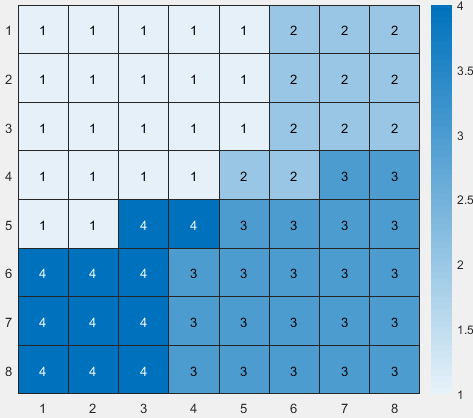
\includegraphics[width=3in]{non-JT_scenario.PNG}
%        \caption{AP assignments in case of Non-JT }
%        \label{fig:non-JT_scenario}
%    \end{center}
%\end{figure}

\begin{table}[h]
    \centering
    \renewcommand{\arraystretch}{1.35}
    \begin{tabular}{|p{2.5cm}||p{2cm}|p{2cm}|p{2cm}|p{2cm}|p{2cm}|}
        \hline
        \multicolumn{6}{|c|}{$C_{Sys} = 1.9648$ bits/sec/Hz,\hspace{0.5cm}    $\sigma^2_{C_{User}} = 0.0001$}
        \\
        \hline\hline
        a & $AP_1^1$ & $AP_1^2$ & $AP_1^3$ & $AP_2^3$ & $\{AP_1^3, AP_2^3\}$ \\
        \hline\hline
        $C_{AP}^S(a)/C_{AP}^J(a)$ & 10.456 & 5.35211 & 10.456 & 5.30628 & -
        \\
        \hline
        $C_{User}^a$ & 0.49791 & 0.48656 & 0.49791 & 0.48656 & -
        \\
        \hline
        $N_S(a)$ & 21 & 11 & 21 & 11 & -
        \\
        \hline
    \end{tabular}
    \caption{non-JT results}
    \label{tab:non-JT_results}
\end{table}

%\begin{figure}[H]
%    \begin{center}
%        \includegraphics[width=7in]{Non-JT_capacity.JPG}
%        \caption{Capacity achieved in non-JT AP assignments }
%        \label{fig:non-JT_results}
%    \end{center}
%\end{figure}




\subsection{With JT-TC}
When the APs in the set $I_3$ are capable of going JT-TC as well as SAPI transmission.
It is expected that with the addition of JT, the overall throughput of the system would increase and STAs situated far away from the APs would be served using JT-TC.

We observed that most of the tiles getting served by $ AP_1^3$ and/or $AP_2^3$ are scheduled to be served in JT mode.
The total average output of the system increases to 2.4876 bits/sec/Hz with a variance of 0.0007 in the average capacity provided to different STAs.
The Figure~\ref{fig:JT} shows the APs assigned to all the STAs in different modes for the best schedule in the JT scenario.

\begin{table}[h]
    \centering
    \renewcommand{\arraystretch}{1.35}
    \begin{tabular}{|p{2.5cm}||p{2cm}|p{2cm}|p{2cm}|p{2cm}|p{2cm}|}
        \hline
        \multicolumn{6}{|c|}{$C_{Sys} = 2.4876$ bits/sec/Hz,\hspace{0.5cm}    $\sigma^2_{C_{User}} = 0.0007$}
        \\
        \hline\hline
        a & $AP_1^1$ & $AP_1^2$ & $AP_1^3$ & $AP_2^3$ & $\{AP_1^3, AP_2^3\}$ \\
        \hline\hline
        $C_{AP}^S(a)/C_{AP}^J(a)$ & 10.456 & 9.99827 & 10.456 & 10.0145 & 11.3172
        \\
        \hline
        $C_{User}^a$ & 0.49791 & 0.47597 & 0.49791 & 0.47688 & 0.53891
        \\
        \hline
        $N_S(a)$ & 21 & 21 & 21 & 21 & -
        \\
        \hline
    \end{tabular}
    \caption{JT results}
    \label{tab:JT_results}
\end{table}

%\begin{figure}[!]
 %   \begin{center}
%        \includegraphics[width=7in]{JT_capacity.JPG}
%        \caption{JT capacity achieved}
%        \label{fig:JT_results}
%    \end{center}
%\end{figure}






% Figure showing schedules for different scenarios
\begin{figure*}[h]
	\centering
	\begin{subfigure}[t]{0.4\linewidth}
		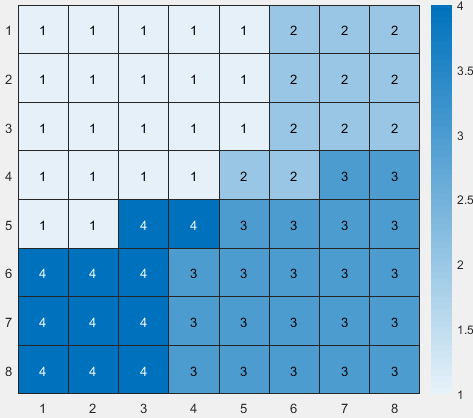
\includegraphics[width=\linewidth]{non-JT_scenario.PNG}
		\caption{non-JT \label{fig:non-JT}} %caption for sub figure 1
        
	\end{subfigure}
	\begin{subfigure}[t]{0.4\linewidth}
		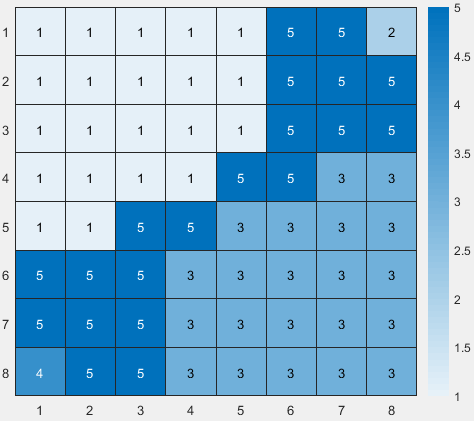
\includegraphics[width=\linewidth]{JT_scenario.PNG}
		\caption{JT \label{fig:JT}} %caption for sub figure 2
       
	\end{subfigure}
	\caption[AP assignments]{AP assignments}
	\label{fig:ap_assignment}
\end{figure*}

It can be clearly seen that enabling Joint Transmission will provide better overall throughput for the system. This mechanism can be especially useful in a big enterprise scenario where many AP work together and have to share channels. It will provide better noise and interference resistance for a far situated user and equalize the individual throughput received in a large area, and provide better channel usage.


%sixth section



\section{Conclusion}
\label{sec:conclusion}

We analysed Joint Transmission and its effect on a multi-AP 802.11be system. We address the problem of assigning the STAs to different APs, while explicitly incorporating the different modes of serving an STA. We provide a mathematical framework to model the scheduling constraints arising from the possibility of including the joint transmission mechanism of serving an STA. We then propose an online algorithm that attempts to achieve a high system level throughput under an inter-STA and inter-AP fairness criterion. We provided the simulation results for this that were done in MATLAB using the wlan toolbox. This algorithm assumes a structure on the various sets involved in the proposed mathematical framework. While using the general mathematical framework developed in the paper, we will now be working on removing the assumptions used in the algorithm.


\appendix
\appendixpage
\section{Proof of the Theorem \ref{theo:rate_JT}}
\label{proof:theo:rate_JT}
The distribution of $\gamma|_{r, h_1,h_2}$ given in \eqref{eq:sinr_jt} can be derived by using the linear combination property of exponential random variables (with mean $\lambda$), $Z=\kappa_1 X+\kappa_2 Y$,  

\begin{equation}
f_Z(z)  = \begin{cases}
\displaystyle\frac{\lambda}{\kappa_1-\kappa_2}\left(e^{-\lambda z /\kappa_1}-e^{-\lambda z /\kappa_2}\right) &; \kappa_1\neq \kappa_2\\\\
\displaystyle\frac{\lambda^2}{a^2} z e^{\frac{-\lambda z}{a}} &; \kappa_1= \kappa_2.
\end{cases}
\label{eq:combined_distribution}
\end{equation}

Since $h_1, h_2$  are Rayleigh fading with unit variance, using notations (for convenience) $a=P_1 r_1^{-\alpha}$ and $b=P_2 r_2^{-\alpha}$ the distribution of $\gamma$ is given by,
\begin{equation}
f_\gamma(\gamma)  = \begin{cases}
\displaystyle\frac{\sigma^2}{a - b}\left[e^{-\gamma\sigma^2/ a}- e^{-\gamma\sigma^2 / b}\right] &; a\neq b\\\\
\displaystyle\frac{\sigma ^4 \gamma   e^{-\frac{\gamma  \sigma ^2 }{a}}}{a^2} &; a= b.
\end{cases}
\label{eq:pdf_gamma}
\end{equation}
Substitute \eqref{eq:pdf_gamma} in \eqref{eq:JT_Cap} and take the expectation the proof is complete.




\section{Proof of Theorem \ref{Theo:SAP_with_interf} }\label{App:theo_SAP}
\begin{proof}
	We have for a positive random variable $X$, $\E(X)=\int_{0}^{\infty}\P(X>t)\text{dt}$. Using the fact that the rate, $R=\log_2(1+\text{SINR})$, is always positive, we can write $\E(R)=\int_{0}^{\infty}\P\left[\text{SINR}>2^t-1\right] \text{dt}$.
	
	The $\text{SINR}$ in this case is given by,
	\[
	\gamma|_{r_1,r_2,h_1,h_2}=\frac{P_1|h_1|^2r_1^{-\alpha}}{\sigma^2+P_2|h_2|^2r_2^{-\alpha}}
	\]
	
	\begin{align}\label{eqn:deri_jt_inter}
	\P[\text{SINR}>z]&=\P\left[|h_1|^2>\frac{zr_1^{\alpha}}{P_1}\left(\sigma^2+P_2|h_2|^2r_2^{-\alpha}\right)\right]\nonumber\\
	&\stackrel{(a)}{=}\E_{h}\left[\exp\left(-\frac{zr_1^{\alpha}}{P_1}\left(\sigma^2+P_2|h_2|^2r_2^{-\alpha}\right)\right)\right]\nonumber\\
	&\stackrel{(b)}{=}\E_{h}\left[e^{-zr_1^{\alpha}\sigma^2/P_1}\exp\left(-|h_2|^2z\frac{P_2r_1^{\alpha}}{P_1 r_2^{\alpha}}\right)\right]\nonumber\\
	&=e^{-zr_1^{\alpha}\sigma^2/P_1}\left(\frac{1}{1+z\frac{P_2r_2^{-\alpha}}{P_1 r_1^{-\alpha}}}\right)
	\end{align}
	The step (a) is using the tail probability of exponential distribution\footnote{$\P(X>\theta)=\exp(-\theta)$ if $X\sim \exp(1).$} and step (b) is by using the Laplace transform of exponential distribution\footnote{$\text{L}_X(s)=\E(\exp(-sX))$, when $X\sim\exp(1)$, $\text{L}(s)=1/(1+s)$}. 
	
	Now by using the property of positive random variables, the proof is complete.
	
	
	
\end{proof}

\section{Proof of Theorem \ref{the:cap_MIMO_JT} }\label{proof:theorem-ber-jt-mimo}

%\thispagestyle{empty}
The squared absolute value  of diagonal elements of the $\text{LQ}$ decomposition of a Rayleigh matrix of order $N \times N$, $|l_{ii}|^2$ is $\Gamma(N-i+1,1)$ distributed
\footnote{$\Gamma(\alpha,\beta)$ is the Gamma distribution with shape parameter $\alpha$ and scale parameter $\beta$. The pdf of Gamma distribution is given by,
$f(x;\alpha,\beta) = \frac{\beta^\alpha x^{\alpha-1}e^{-\beta x}}{\Gamma(\alpha)}, x>0, \alpha,\beta >0,
$}.
Here the channel coefficient are scaled by pathloss, $r_j^{-\alpha/2}$, therefor, $|l_{ii}^{(j)}|^2$ will be scaled by $r_j^{-\alpha}$. 

% \begin{equation}
%     \textcolor{red}{\sum\limits_{a \in S(x,y); i < C} N_a^S + \sum\limits_{a \in S(x,y); i>C^*} N_a^{JT} = T}
% \end{equation}

The distribution of $\gamma_{i}^{JTM}$ given in \eqref{eqn:SNR_JT_MIMO} can be derived by using the linear combination property of random variables, $Z=a X+b Y$, i.e., 
\[f_Z(z) = \frac{1}{ab} \int_{0}^{z} f_X(x/a) f_Y((z-x)/b) \text{dx}\]
Therefore,
\begin{align}
    \label{eqn:deri_fZz_JTMIMO}
    %f_{\gamma_i}(z)&=\frac{1}{ab}\int_{0}^{z} \frac{(x/a)^{N-i}e^{-x/a}}{(N-i)!} \frac{((z-x)/b)^{N-i}e^{-(z-x)/b}}{(N-i)!}\d x,\nonumber\\
    %&=\frac{1}{(ab)^{N+1}(N!)^2}\int_{0}^{z} x^{N}e^{-x/a} (z-x)^{N}e^{-(z-x)/b}\d x,\nonumber\\
    %&=\frac{1}{(ab)^{N+1}(N!)^2}\int_{0}^{z} x^{N}e^{-\frac{x}{a}} (z-x)^{N}e^{-\frac{z-x}{b}}\d x,\nonumber\\
    f_{\gamma_i}(z) =& \frac{e^{-z/b}}{(ab)^{N-i+1}((N-i)!)^2}\nonumber\\
    &\times\int_{0}^{z} x^{N-i}(z-x)^{N-i} e^{-x\beta}\d x\nonumber\\
%    &\stackrel{(a)}{=}\frac{e^{-z/b}}{(ab)^{N+1}(N!)^2}\int_{0}^{z} x^{N} e^{-x\beta}\sum_{l=0}^{N} {N \choose l}(-1)^l x^l  z^{N-l}\d x\nonumber\\
%    &=\frac{e^{-z/b}}{(ab)^{N+1}(N!)^2} \sum_{l=0}^{N} {N \choose l}(-1)^l  z^{N-l}\int_{0}^{z} x^{N+l}  e^{-x\beta}\d x\nonumber\\
%    &=\frac{e^{-z/b}z^{N}}{(ab)^{N+1}(N!)^2} \sum_{l=0}^{N} {N \choose l}(-1)^l  z^{-l} z^{l+N+1} (\beta  z)^{-l-N-1} (\Gamma (l+N+1)-\Gamma (l+N+1,z
%    \beta )) \nonumber\\
%    &=\frac{e^{-z/b}z^{2N+1}(\beta  z)^{-N-1}}{(ab)^{N+1}(N!)^2} \sum_{l=0}^{N} {N \choose l}(-1)^l    \frac{(\Gamma (l+N+1)-\Gamma (l+N+1,z
%    	\beta ))}{(\beta  z)^{l}} \nonumber\\
%    &\stackrel{(a)}{=}\frac{e^{-z/b}z^{2N+1}(\beta  z)^{-N-1}}{(ab)^{N+1}(N!)^2} \sum_{l=0}^{N} {N \choose l}\left(-1\right)^l  \frac{\Lambda_{\beta}(z,l+N+1)}{(\beta  z)^{l}}   \nonumber\\
    \stackrel{(a)}{=}& \frac{e^{-z/b}z^{N-i}}{(b-a)^{N-i+1}((N-i)!)^2} \nonumber\\
    &\times\sum_{l=0}^{N-i} {N-i \choose l}  \frac{\left(-1\right)^l\Lambda_{\beta}(z,l+N-i+1)}{(\beta  z)^{l}}
\end{align}
where  $a=P_1r_1^{-\alpha}/\sigma^2$, $b=P_2r_2^{-\alpha}/\sigma^2$,  $\beta=1/a-1/b$. The step (a) is by substituting the binomial expansion of $(z-x)^{N}$ and $\Lambda_{\beta}(z,k)$ is given by,
\begin{align}\label{eqn:Lambda_def}
\Lambda_{\beta}(z,k) =(\Gamma (k)-\Gamma (k,z
\beta ))
\end{align}
The distribution of $\gamma_{i}$ for $a=b$, can be derived in a similar way by using the linear combination property of random variables, i.e., when  $Z=a (X+ Y)=a S$, we have, 
$f_Z(z) = \frac{1}{a} f_S(s/a)$ and $f_S(s) = \int_{0}^{s} f_X(x) f_Y(s-x) \d x$. 
%\begin{align}
%f_S(s) &= \int_{0}^{s} f_X(x) f_Y(s-x) \d x \nonumber\\
%&=\int_{0}^{s}\frac{x^{N-i} e^{-x} (s-x)^{N-i} e^{-(s-x)}}{(N-i)!(N-i)!}\d x\nonumber\\
%&=\frac{e^{-s}}{(N-i)!(N-i)!}\int_{0}^{s}x^{N-i} (s-x)^{N-i} \d x\nonumber\\
%&=\frac{e^{-s}}{(N-i)!(N-i)!}\sum_{l=0}^{N-i} {N-i \choose l}(-1)^{l}(s)^{l}\int_{0}^{s}x^{2N-2i-l} \d x\nonumber\\
%&=\frac{e^{-s}s^{2N-2i+1}}{(N-i)!(N-i)!}\sum_{l=0}^{N-i} {N-i \choose l}\frac{(-1)^{l}}{2N-2i-l+1}\nonumber\\
%\end{align}
\begin{align}\label{eqn:deri_fZz_JTMIMO_2}
    f_{\gamma_{i}}(z) &= \frac{(a^2)^{N-i}e^{-z/a}z(z^2)^{N-i}}{(N-i)!(N-i)!}\sum_{l=0}^{N-i} {N-i \choose l}\frac{(-1)^{l}}{2N-2i-l+1}
\end{align}
%Then the rate of $i^{th}$ stream,
%\begin{align}
%    \E(R_i) =\frac{(a^2)^{N-i}}{((N-i)!)^2} \sum_{l=0}^{N-i}\frac{{N-i \choose l}(-1)^{l} \int_{0}^{\infty} \log_2(1+z)e^{-z/a}z(z^2)^{N-i} \d z}{2(N-i)-l+1}\nonumber\\
%\end{align}
now by substituting \eqref{eqn:deri_fZz_JTMIMO}, \eqref{eqn:deri_fZz_JTMIMO_2}, in \eqref{eqn:per_stream_rate}, proof is complete.

\bibliographystyle{unsrt}
\bibliography{references}



% Text with citations \cite{RefB} and \cite{RefJ}.
% \subsection{Subsection title}
% \label{sec:2}
% as required. Don't forget to give each section
% and subsection a unique label (see Sect.~\ref{sec:1}).
% \paragraph{Paragraph headings} Use paragraph headings as needed.
% \begin{equation}
% a^2+b^2=c^2
% \end{equation}

% % For one-column wide figures use
% \begin{figure}
% % Use the relevant command to insert your figure file.
% % For example, with the graphicx package use
%   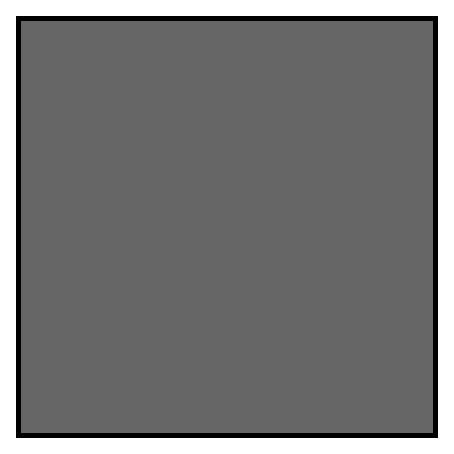
\includegraphics{example.eps}
% % figure caption is below the figure
% \caption{Please write your figure caption here}
% \label{fig:1}       % Give a unique label
% \end{figure}
%
% % For two-column wide figures use
% \begin{figure*}
% % Use the relevant command to insert your figure file.
% % For example, with the graphicx package use
%   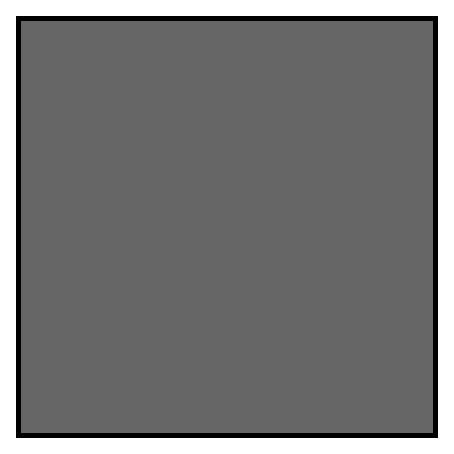
\includegraphics[width=0.75\textwidth]{example.eps}
% % figure caption is below the figure
% \caption{Please write your figure caption here}
% \label{fig:2}       % Give a unique label
% \end{figure*}
%
% For tables use
% \begin{table}
% % table caption is above the table
% \caption{Please write your table caption here}
% \label{tab:1}       % Give a unique label
% % For LaTeX tables use
% \begin{tabular}{lll}
% \hline\noalign{\smallskip}
% first & second & third  \\
% \noalign{\smallskip}\hline\noalign{\smallskip}
% number & number & number \\
% number & number & number \\
% \noalign{\smallskip}\hline
% \end{tabular}
% \end{table}


%\begin{acknowledgements}
%If you'd like to thank anyone, place your comments here
%and remove the percent signs.
%\end{acknowledgements}


% Authors must disclose all relationships or interests that 
% could have direct or potential influence or impart bias on 
% the work: 
%
% \section*{Conflict of interest}
%
% The authors declare that they have no conflict of interest.


% BibTeX users please use one of
%\bibliographystyle{spbasic}      % basic style, author-year citations
%\bibliographystyle{spmpsci}      % mathematics and physical sciences
%\bibliographystyle{spphys}       % APS-like style for physics
%\bibliography{}   % name your BibTeX data base

% Non-BibTeX users please use
% \begin{thebibliography}{}
% %
% % and use \bibitem to create references. Consult the Instructions
% % for authors for reference list style.
% %
% \bibitem{RefJ}
% % Format for Journal Reference
% Author, Article title, Journal, Volume, page numbers (year)
% % Format for books
% \bibitem{RefB}
% Author, Book title, page numbers. Publisher, place (year)
% % etc
% \end{thebibliography}

\end{document}
% end of file template.tex

